\documentclass[11pt,oneside]{article}    %use"amsart"insteadof"article"forAMSLaTeXformat
\usepackage{geometry}        %Seegeometry.pdftolearnthelayoutoptions.Therearelots.
\geometry{letterpaper}        %...ora4paperora5paperor...
%\geometry{landscape}        %Activateforforrotatedpagegeometry
%\usepackage[parfill]{parskip}        %Activatetobeginparagraphswithanemptylineratherthananindent
\usepackage{graphicx}                %Usepdf,png,jpg,orepsßwithpdflatex;useepsinDVImode
                                %TeXwillautomaticallyconverteps-->pdfinpdflatex        
\usepackage{amssymb}
\usepackage[colorlinks]{hyperref}

%----macros begin---------------------------------------------------------------
\usepackage{color}
\usepackage{amsthm}

\def\conv{\mbox{\textrm{conv}\,}}
\def\aff{\mbox{\textrm{aff}\,}}
\def\E{\mathbb{E}}
\def\R{\mathbb{R}}
\def\Z{\mathbb{Z}}
\def\tex{\TeX}
\def\latex{\LaTeX}
\def\v#1{{\bf #1}}
\def\p#1{{\bf #1}}
\def\T#1{{\bf #1}}

\def\vet#1{{\left(\begin{array}{cccccccccccccccccccc}#1\end{array}\right)}}
\def\mat#1{{\left(\begin{array}{cccccccccccccccccccc}#1\end{array}\right)}}

\def\lin{\mbox{\rm lin}\,}
\def\aff{\mbox{\rm aff}\,}
\def\pos{\mbox{\rm pos}\,}
\def\cone{\mbox{\rm cone}\,}
\def\conv{\mbox{\rm conv}\,}
\newcommand{\homog}[0]{\mbox{\rm homog}\,}
\newcommand{\relint}[0]{\mbox{\rm relint}\,}

%----macros end-----------------------------------------------------------------

\title{Accelerated intersection of geometric objects
\footnote{This document is part of the \emph{Linear Algebraic Representation with CoChains} (LAR-CC) framework~\cite{cclar-proj:2013:00}. \today}
}
\author{Alberto Paoluzzi}
%\date{}                            %Activatetodisplayagivendateornodate

\begin{document}
\maketitle
\nonstopmode

\begin{abstract}
This module contains the first experiments of a parallel implementation of the intersection of (multidimensional) geometric objects. The first installment is being oriented to the intersection of line segment in the 2D plane. A generalization of the algorithm, based on the classification of the containment boxes of the geometric values, will follow quickly.
\end{abstract}

\tableofcontents

%===============================================================================
\section{Introduction}
%===============================================================================

An easily parallelizable implementation of the accelerated intersection of geometric objects is given in this module. Our first aim is to implement a specialized version for simplices, that generalizes the $nD$-trees of points (that are 0-simplices), to $(d-1)$-dimensional simplices in $d$-space, starting with the intersection of line segments in the plane. Our plan is to follow with an implementation for intersection of general \emph{non convex} sets.


%===============================================================================
\section{Implementation}
%===============================================================================

The first implementation of this module concerns the computation of the intersection points among a set of line segment in the 2D plane. The containment boxes of the input segments are iteratively classified against the 1-dimensional centroid of smaller and smaller buckets of data. 

At the end of the classification, where the same geometric object may be inserted in several different buckets, a \emph{brute-force} intersection is applied to each final subset. Finally, the duplicated intersection points are removed, and a 1-dimensional LAR data structure is generated, with 1-cells given by the split line segments. 

A complete LAR of the plane partition generated by the arrangment of lines is then computed by: (a) generating the maximal 2-connected components of such 1-dimensional graph; and (b) by traversing in counter-clockwise order the generated subgraphs to report the 2-dimensional cells of the plane partition.

The splitting algorithm may be easily parallelized, since both during their generation and at the end of this one, the various buckets of data can be dispatched to different processors for independent computation, followed by elimination of duplicates. In particular, a standard \emph{map-reduce} software infrastructure may be used for this parallelization purpose.


\subsection{Construction of independent buckets}
%===============================================================================


\paragraph{Containment boxes}

Given as input a list \texttt{randomLineArray} of pairs of 2D points, the function \texttt{containment2DBoxes} returns, in the same order, the list of \emph{containment boxes} of the input lines. A \emph{containment box} of a geometric object of dimension $d$ is defined as the minimal $d$-cuboid, equioriented with the reference frame, that contains the object. For a 2D line it is given by the tuple $(x1,y1,x2,y2)$, where $(x1,y1)$ is the point of minimal coordinates, and $(x2,y2)$ is the point of maximal  coordinates.

%-------------------------------------------------------------------------------
@D Containment boxes
@{""" Containment boxes """
def containment2DBoxes(randomLineArray):
    boxes = [eval(vcode([min(x1,x2),min(y1,y2),max(x1,x2),max(y1,y2)]))
            for ((x1,y1),(x2,y2)) in randomLineArray]
    return boxes
@}
%-------------------------------------------------------------------------------



\paragraph{Splitting the input above and below a threshold}
%-------------------------------------------------------------------------------
@D Splitting the input above and below a threshold
@{""" Splitting the input above and below a threshold """
def splitOnThreshold(boxes,subset,coord):
    theBoxes = [boxes[k] for k in subset]
    threshold = centroid(theBoxes,coord)
    ncoords = len(boxes[0])/2
    a = coord%ncoords
    b = a+ncoords
    below,above = [],[]
    for k in subset:
        if boxes[k][a] <= threshold: below += [k]
    for k in subset:
        if boxes[k][b] >= threshold: above += [k]
    return below,above
@}
%-------------------------------------------------------------------------------


\paragraph{Iterative splitting of box buckets}
%-------------------------------------------------------------------------------
@D Iterative splitting of box buckets
@{""" Iterative splitting of box buckets """
def splitting(bucket,below,above, finalBuckets,splittingStack):
    if (len(below)<4 and len(above)<4) or len(set(bucket).difference(below))<7 \
        or len(set(bucket).difference(above))<7: 
        finalBuckets.append(below)
        finalBuckets.append(above)
    else: 
        splittingStack.append(below)
        splittingStack.append(above)

def geomPartitionate(boxes,buckets):
    geomInters = [set() for h in range(len(boxes))]
    for bucket in buckets:
        for k in bucket:
            geomInters[k] = geomInters[k].union(bucket)
    for h,inters in enumerate(geomInters):
        geomInters[h] = geomInters[h].difference([h])
    return AA(list)(geomInters)

def boxBuckets(boxes):
    bucket = range(len(boxes))
    splittingStack = [bucket]
    finalBuckets = []
    while splittingStack != []:
        bucket = splittingStack.pop()
        below,above = splitOnThreshold(boxes,bucket,1)
        below1,above1 = splitOnThreshold(boxes,above,2)
        below2,above2 = splitOnThreshold(boxes,below,2)                      
        splitting(above,below1,above1, finalBuckets,splittingStack)
        splitting(below,below2,above2, finalBuckets,splittingStack)      
        finalBuckets = list(set(AA(tuple)(finalBuckets)))
    parts = geomPartitionate(boxes,finalBuckets)
    return AA(sorted)(parts)
    #return finalBuckets
@}
%-------------------------------------------------------------------------------


\subsection{Brute force intersection within the buckets}
%===============================================================================




\paragraph{Intersection of two line segments}
%-------------------------------------------------------------------------------
@D Intersection of two line segments
@{""" Intersection of two line segments """
def segmentIntersect(boxes,lineArray,pointStorage):
    def segmentIntersect0(h):
        p1,p2 = lineArray[h]
        line1 = '['+ vcode(p1) +','+ vcode(p2) +']'
        (x1,y1),(x2,y2) = p1,p2
        B1,B2,B3,B4 = boxes[h]
        def segmentIntersect1(k):
            p3,p4 = lineArray[k]
            line2 = '['+ vcode(p3) +','+ vcode(p4) +']'
            (x3,y3),(x4,y4) = p3,p4
            b1,b2,b3,b4 = boxes[k]
            if not (b3<B1 or B3<b1 or b4<B2 or B4<b2):
            #if True:
                m23 = mat([p2,p3])
                m14 = mat([p1,p4])
                m = m23 - m14
                v3 = mat([p3])
                v1 = mat([p1])
                v = v3-v1
                a=m[0,0]; b=m[0,1]; c=m[1,0]; d=m[1,1];
                det = a*d-b*c
                if det != 0:
                    m_inv = mat([[d,-b],[-c,a]])*(1./det)
                    alpha, beta = (v*m_inv).tolist()[0]
                    #alpha, beta = (v*m.I).tolist()[0]
                    if -0.0<=alpha<=1 and -0.0<=beta<=1:
                        pointStorage[line1] += [alpha]
                        pointStorage[line2] += [beta]
                        return list(array(p1)+alpha*(array(p2)-array(p1)))
            return None
        return segmentIntersect1
    return segmentIntersect0
@}
%-------------------------------------------------------------------------------


\paragraph{Brute force bucket intersection}
%-------------------------------------------------------------------------------
@D Brute force bucket intersection
@{""" Brute force bucket intersection """
def lineBucketIntersect(boxes,lineArray, h,bucket, pointStorage):
    intersect0 = segmentIntersect(boxes,lineArray,pointStorage)
    intersectionPoints = []
    intersect1 = intersect0(h)
    for line in bucket:
        point = intersect1(line)
        if point != None: 
            intersectionPoints.append(eval(vcode(point)))
    return intersectionPoints
@}
%-------------------------------------------------------------------------------


\paragraph{Accelerate intersection of lines}
%-------------------------------------------------------------------------------
@D Accelerate intersection of lines
@{""" Accelerate intersection of lines """
def lineIntersection(lineArray):
    lineArray = [line for line in lineArray if len(line)>1]

    from collections import defaultdict
    pointStorage = defaultdict(list)
    for line in lineArray:
        p1,p2 = line
        key = '['+ vcode(p1) +','+ vcode(p2) +']'
        pointStorage[key] = []

    boxes = containment2DBoxes(lineArray)
    buckets = boxBuckets(boxes)
    intersectionPoints = set()
    for h,bucket in enumerate(buckets):
        pointBucket = lineBucketIntersect(boxes,lineArray, h,bucket, pointStorage)
        intersectionPoints = intersectionPoints.union(AA(tuple)(pointBucket))

    frags = AA(eval)(pointStorage.keys())
    params = AA(COMP([sorted,list,set,tuple,eval,vcode]))(pointStorage.values())
        
    return intersectionPoints,params,frags  ### GOOD: 1, WRONG: 2 !!!
@}
%-------------------------------------------------------------------------------


\subsection{Generation of LAR representation of split segments}
%===============================================================================
The function \texttt{lines2lar} is used to generate a 1-dimensional LAR complex from
an array of lines, i.e.~of pairs of 2D points. For every \emph{line} in \texttt{frags}
is computed an \emph{ordered} list \texttt{outline} of \emph{symbolic} intersection points, including 
the first and last vertex of the line, and every interior point generated by the list \texttt{params[k]}.

Then, for every symbolic representation \texttt{key} of a point in \texttt{outline}, a 
dictionary vertex is either created or retrieved, and a corresponding edge is orderly created, using the index of the point.
At the same time, the vertices created in this way are accumulated within the \texttt{V} array.
Finally, each edge in EV is extended to contain a second vertex index using the subsequent edge.  

The third stage finalizes the vertex set of the output LAR, by identifying the closest vertices, i.e.~those at distance
less or equal to the current resolution, set to \texttt{10**(-PRECISION)}, by searching via the \texttt{scipy.spatialKDTree} the pairs of vertices at less than this distance.

A fourth stage identifies the possibly duplicated edges. Some of these could appear, e.g., when importing a set of adjacent boxes from some drawing program, to generate an array of lines, to be mutually intersected and transformed into a LAR data structure.

\paragraph{Create the LAR of fragmented lines}
%-------------------------------------------------------------------------------
@D Create the LAR of fragmented lines
@{""" Create the LAR of fragmented lines """
from scipy import spatial

def lines2lar(lineArray):
    _,params,frags = lineIntersection(lineArray)
    vertDict = dict()
    index,defaultValue,V,EV = -1,-1,[],[]
    
    for k,(p1,p2) in enumerate(frags):
        outline = [vcode(p1)]
        if params[k] != []:
            for alpha in params[k]:
                if alpha != 0.0 and alpha != 1.0:
                    p = list(array(p1)+alpha*(array(p2)-array(p1)))
                    outline += [vcode(p)]
        outline += [vcode(p2)]
    
        edge = []
        for key in outline:
            if vertDict.get(key,defaultValue) == defaultValue:
                index += 1
                vertDict[key] = index
                edge += [index]
                V += [eval(key)]
            else:
                edge += [vertDict[key]]
            EV.extend([[edge[k],edge[k+1]] for k,v in enumerate(edge[:-1])])
    
    model = (V,EV)
    return larSimplify(model)
@}
%-------------------------------------------------------------------------------



\subsection{Biconnected components of a 1-complex}
%===============================================================================

An implementation of the Hopcroft-Tarjan algorithm~\cite{Hopcroft:1973:AEA:362248.362272} for computation of the biconnected components of a graph is given here.



\paragraph{Biconnected components}
%-------------------------------------------------------------------------------
@D Biconnected components
@{""" Biconnected components """
@< Adjacency lists of 1-complex vertices @>
@< Main procedure for biconnected components @>
@< Hopcroft-Tarjan algorithm @>
@< Output of biconnected components @>
@}
%-------------------------------------------------------------------------------



\paragraph{Adjacency lists of 1-complex vertices}
%-------------------------------------------------------------------------------
@D Adjacency lists of 1-complex vertices
@{""" Adjacency lists of 1-complex vertices """
import larcc 
def vertices2vertices(model):
    V,EV = model
    csrEV = larcc.csrCreate(EV)
    csrVE = larcc.csrTranspose(csrEV)
    csrVV = larcc.matrixProduct(csrVE,csrEV)    
    cooVV = csrVV.tocoo()
    data,rows,cols = AA(list)([cooVV.data, cooVV.row, cooVV.col])
    triples = zip(data,rows,cols)
    VV = [[] for k in range(len(V))]
    for datum,row,col in triples:
        if row != col: VV[col] += [row]
    return AA(sorted)(VV)
@}
%-------------------------------------------------------------------------------


\paragraph{Main procedure for biconnected components}
%-------------------------------------------------------------------------------
@D Main procedure for biconnected components
@{""" Main procedure for biconnected components """
def biconnectedComponent(model):
    W,_ = model
    V = range(len(W))
    count = 0
    stack,out = [],[]
    visited = [None for v in V]
    parent = [None for v in V]
    d = [None for v in V]
    low = [None for v in V]
    for u in V: visited[u] = False
    for u in V: parent[u] = []
    VV = vertices2vertices(model)
    for u in V: 
        if not visited[u]: 
            DFV_visit( VV,out,count,visited,parent,d,low,stack, u )
    return W,[component for component in out if len(component) > 1]
@}
%-------------------------------------------------------------------------------


\paragraph{Hopcroft-Tarjan algorithm}
%-------------------------------------------------------------------------------
@D Hopcroft-Tarjan algorithm
@{""" Hopcroft-Tarjan algorithm """
def DFV_visit( VV,out,count,visited,parent,d,low,stack,u ):
    visited[u] = True
    count += 1
    d[u] = count
    low[u] = d[u]
    for v in VV[u]:
        if not visited[v]:
            stack += [(u,v)]
            parent[v] = u
            DFV_visit( VV,out,count,visited,parent,d,low,stack, v )
            if low[v] >= d[u]:
                out += [outputComp(stack,u,v)]
            low[u] = min( low[u], low[v] )
        else:
            if not (parent[u]==v) and (d[v] < d[u]):
                stack += [(u,v)]
                low[u] = min( low[u], d[v] )
@}
%-------------------------------------------------------------------------------


\paragraph{Output of biconnected components}
%-------------------------------------------------------------------------------
@D Output of biconnected components
@{""" Output of biconnected components """
def outputComp(stack,u,v):
    out = []
    while True:
        e = stack.pop()
        out += [list(e)]
        if e == (u,v): break
    return list(set(AA(tuple)(AA(sorted)(out))))
@}
%-------------------------------------------------------------------------------


\begin{figure}[htbp] %  figure placement: here, top, bottom, or page
   \centering
   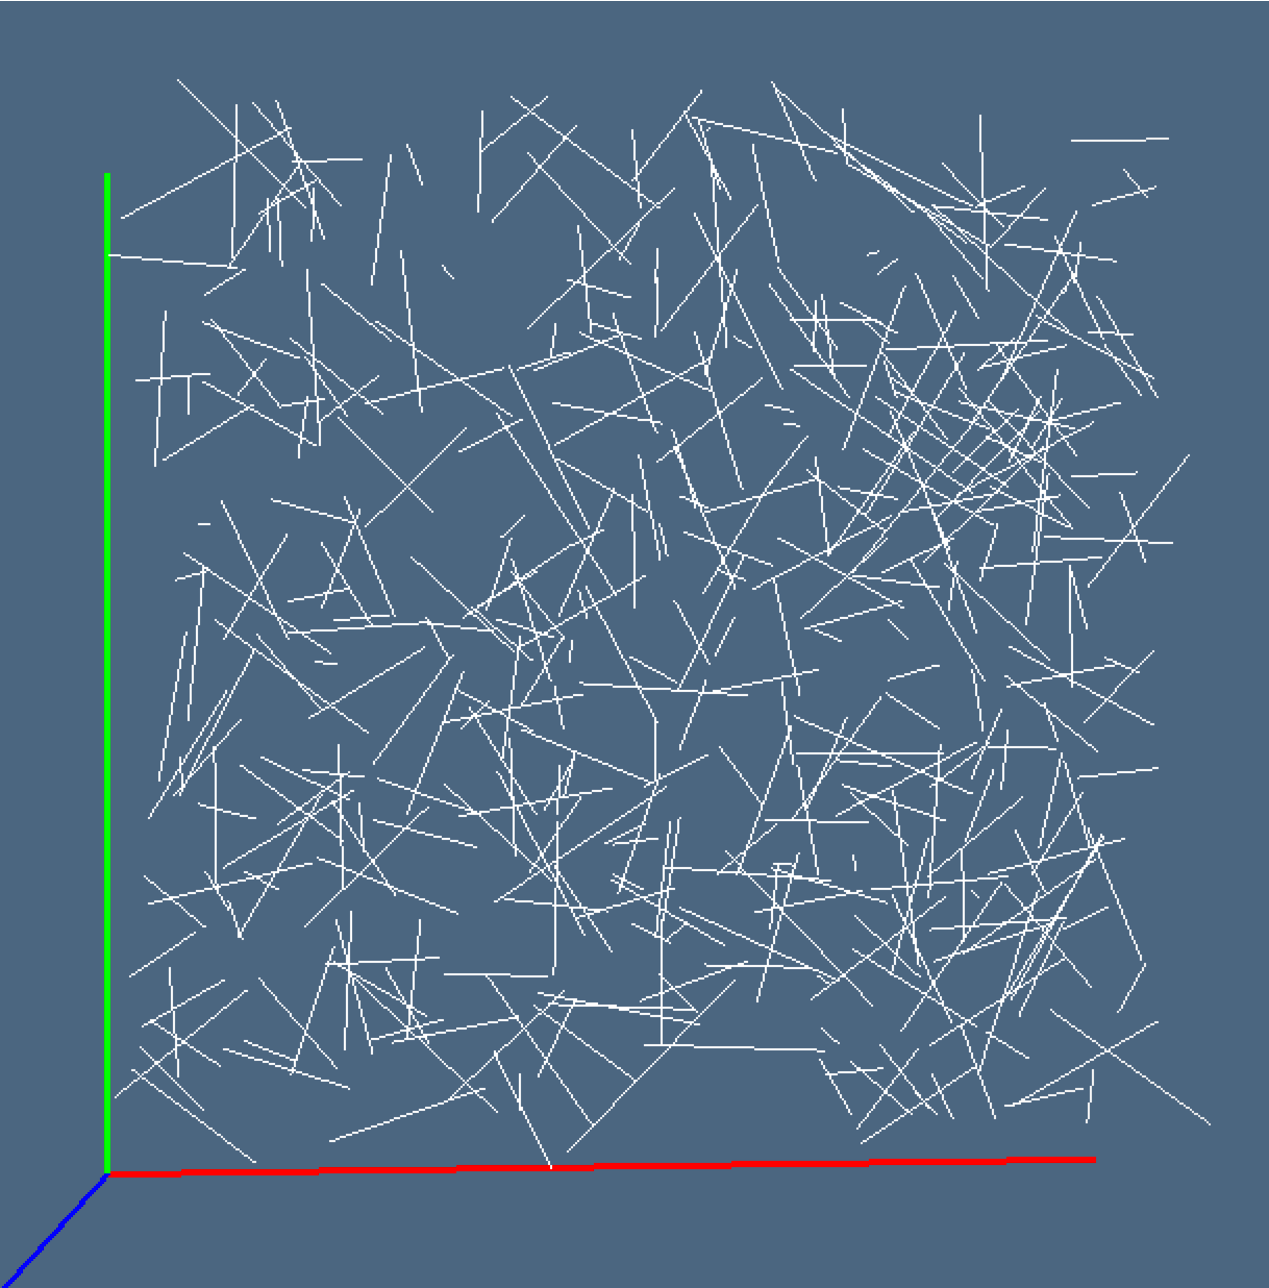
\includegraphics[height=0.49\linewidth,width=0.49\linewidth]{images/biconnected1} 
   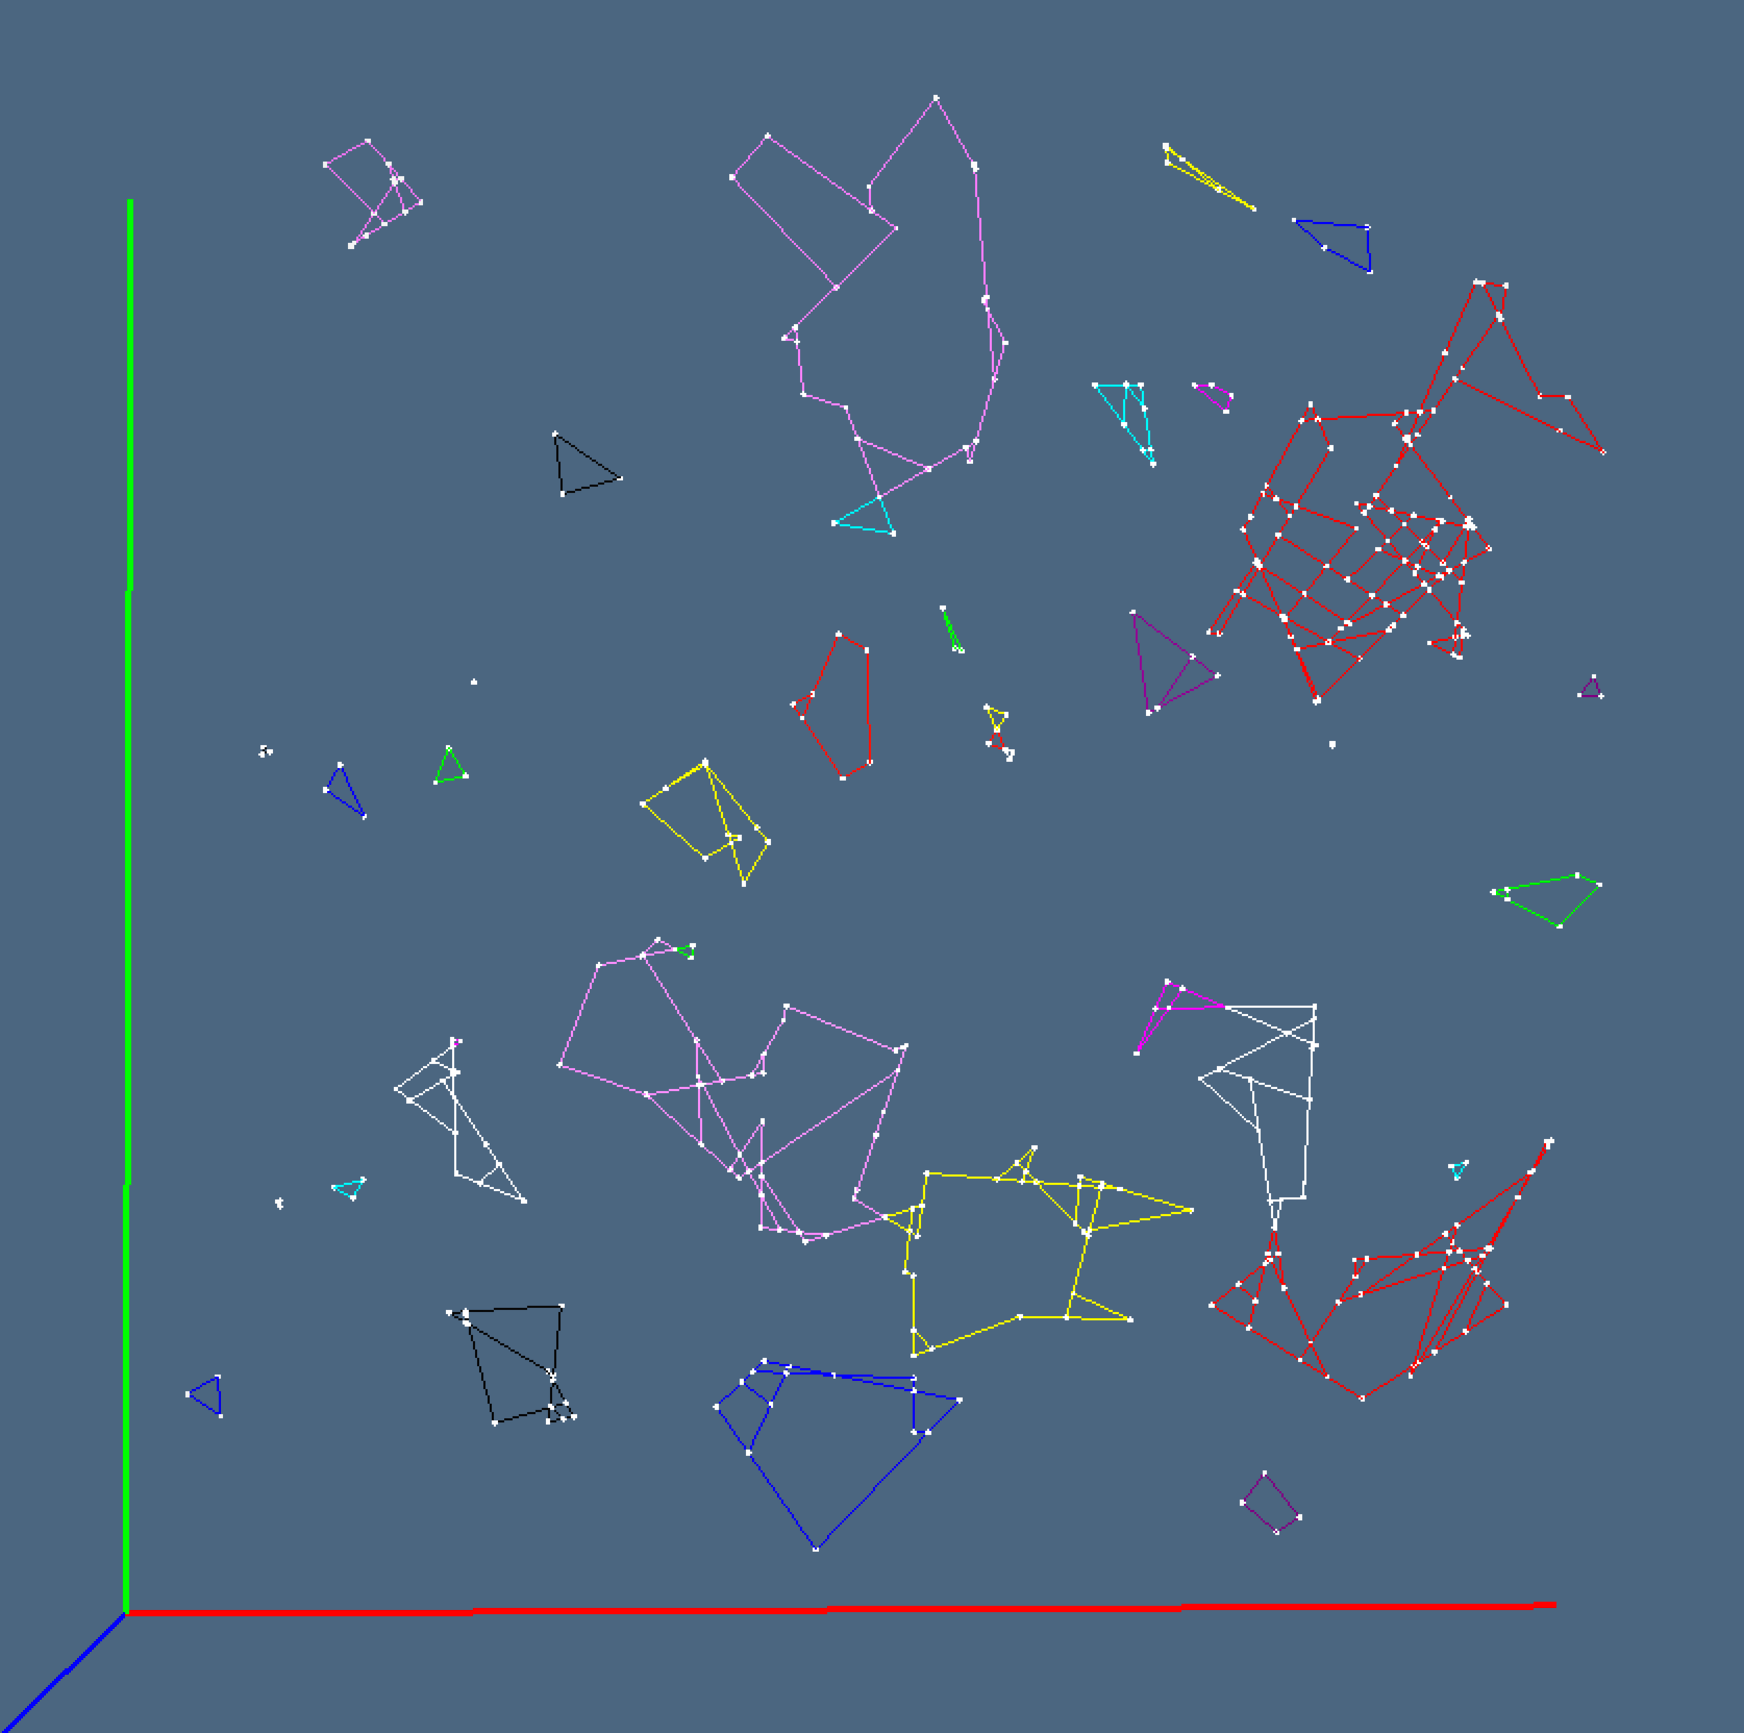
\includegraphics[height=0.49\linewidth,width=0.49\linewidth]{images/biconnected2} 

   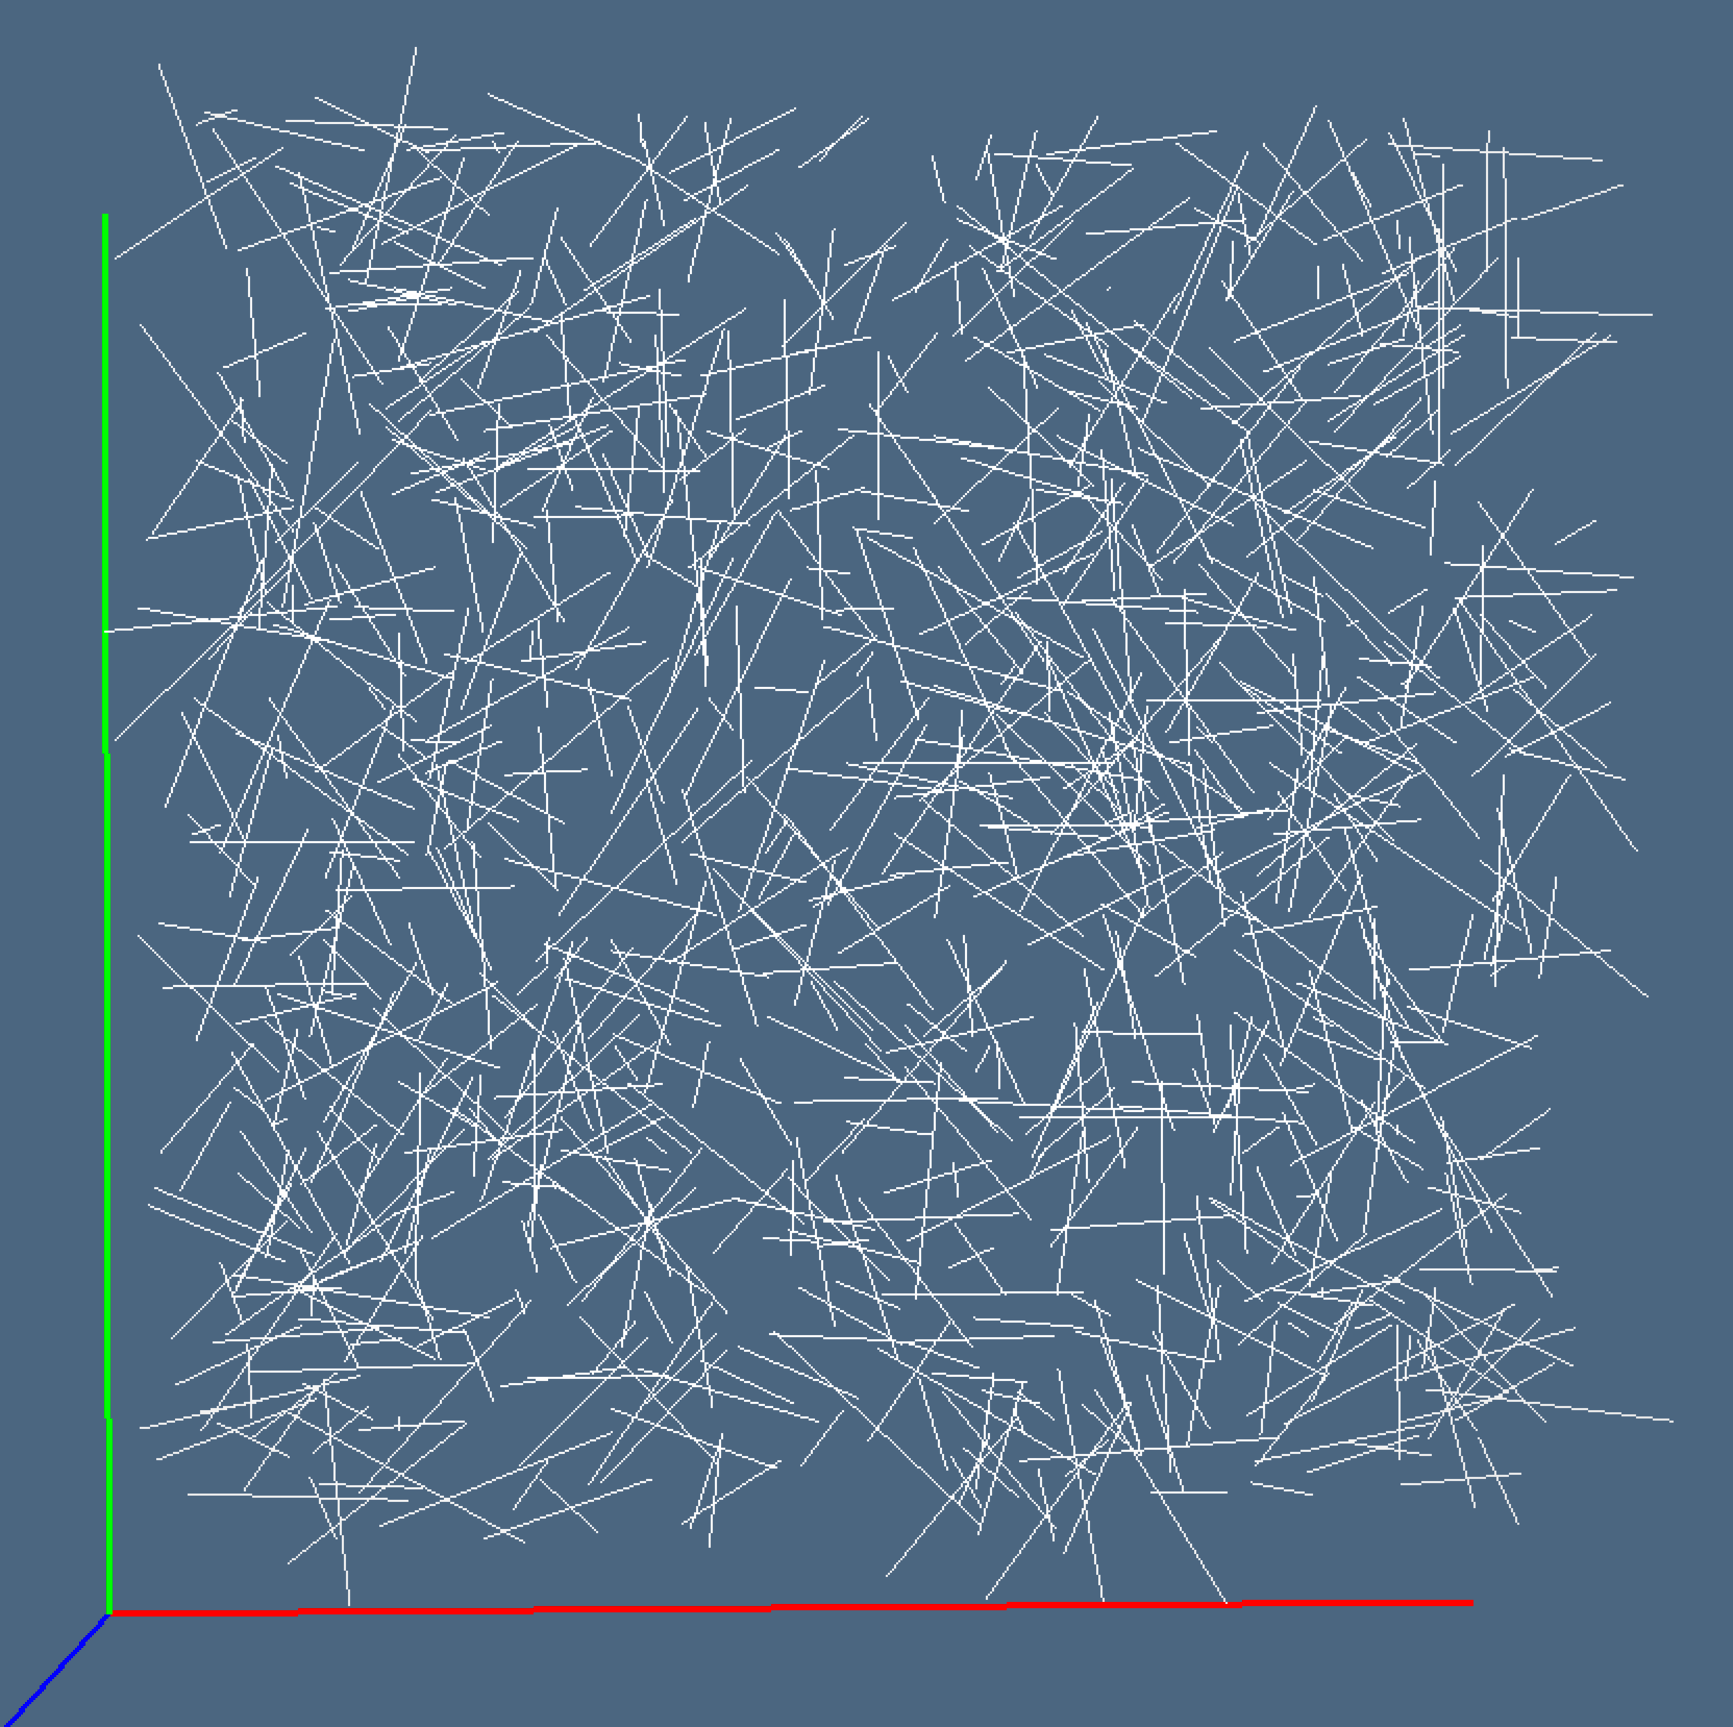
\includegraphics[height=0.49\linewidth,width=0.49\linewidth]{images/biconnected3} 
   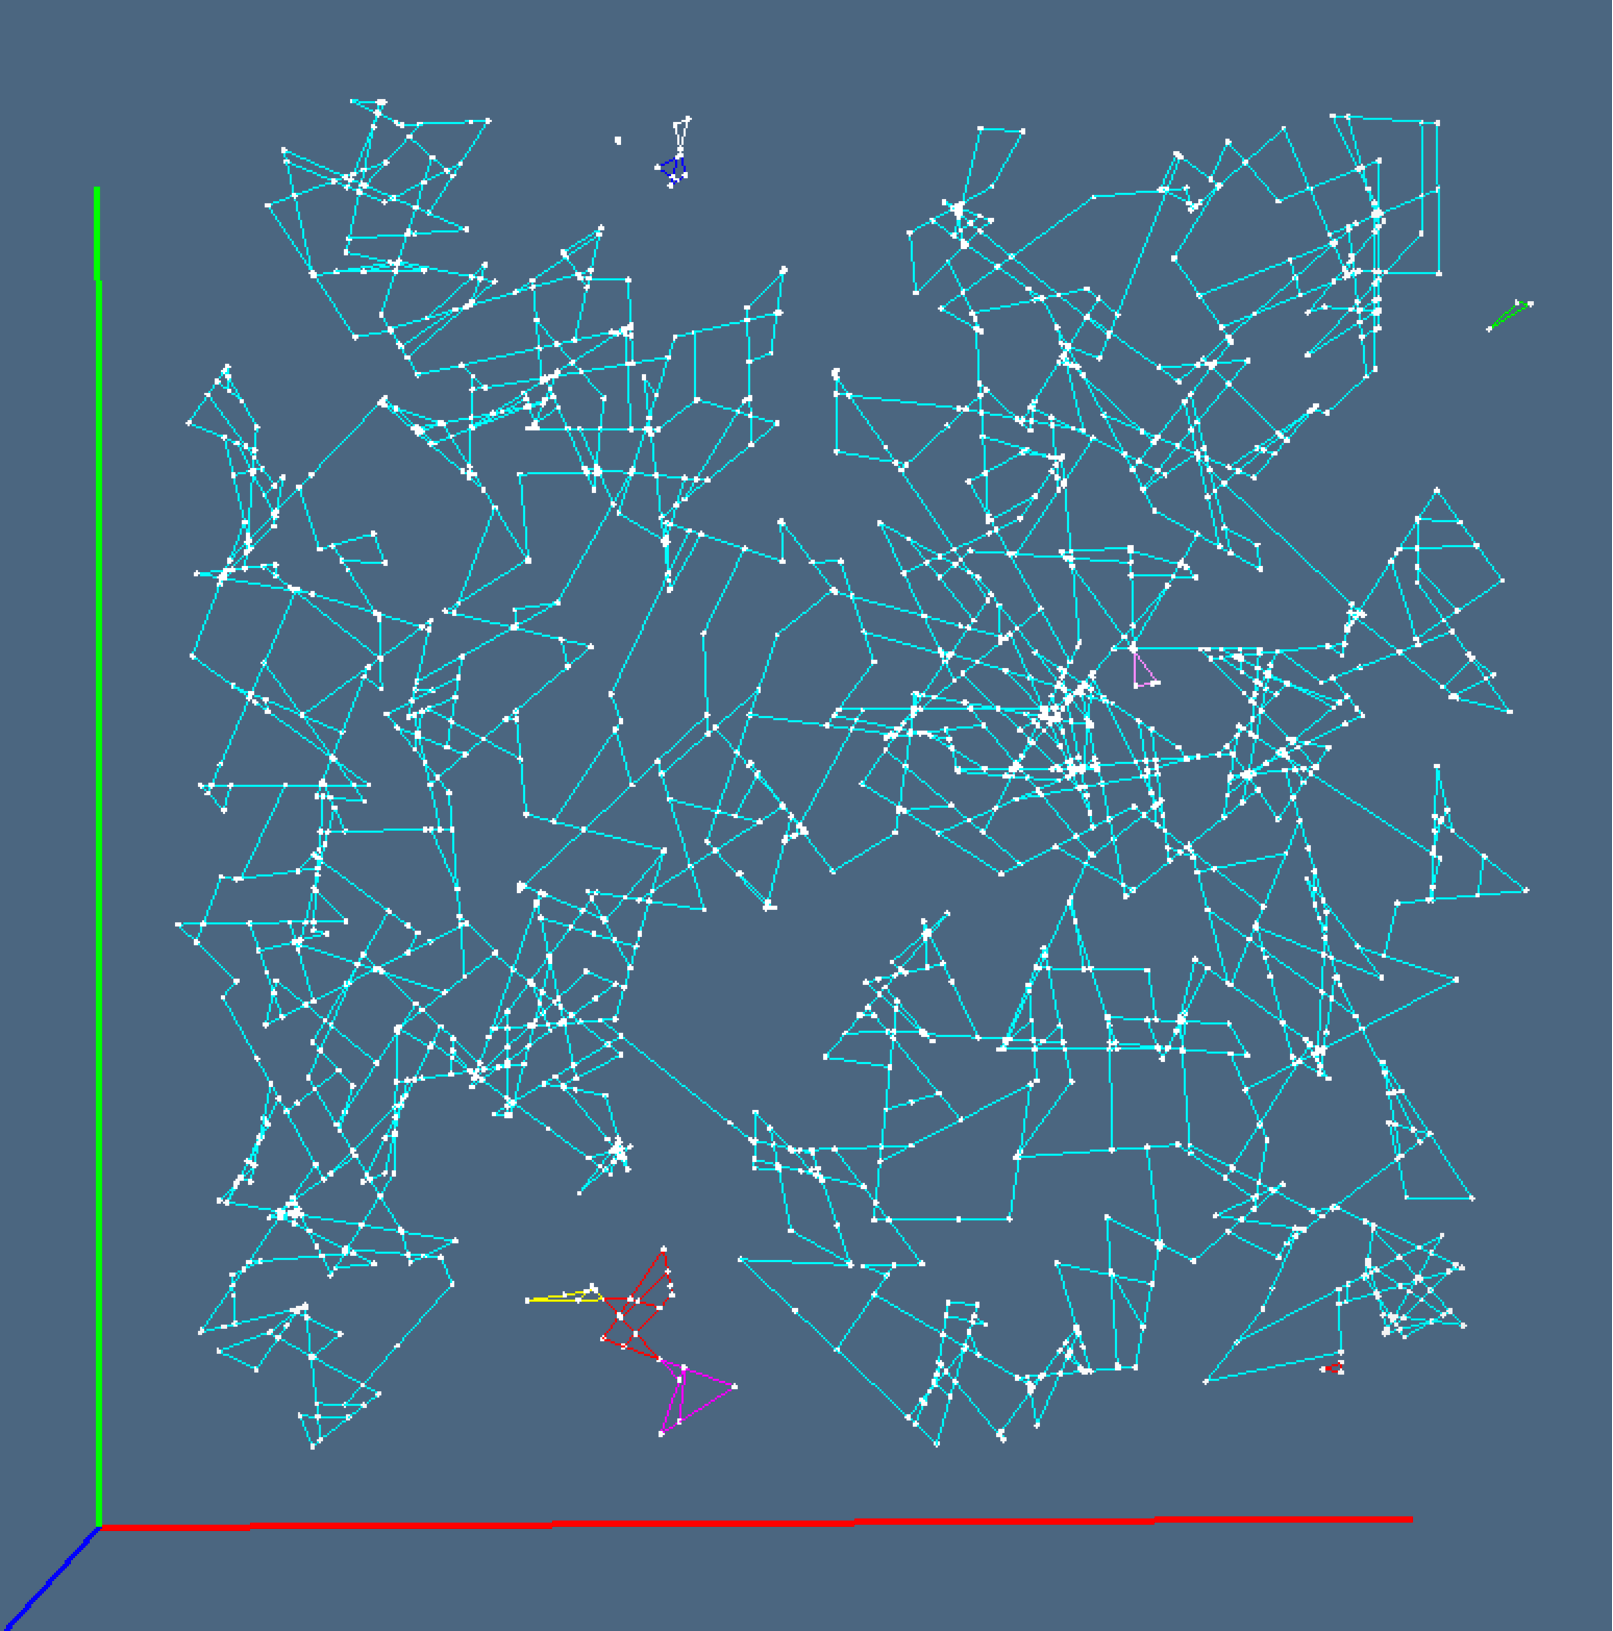
\includegraphics[height=0.49\linewidth,width=0.49\linewidth]{images/biconnected4} 
   \caption{Two random line arrangements, and the biconnected components extracted by their LAR 1-complexes.}
   \label{fig:biconnected}
\end{figure}


\subsection{2D cells from biconnected components}
%===============================================================================

It is very easy,  using the LAR representation of topology, to compute the 2-cells of the plane partitions~(see Figures~\ref{fig:biconnected}b and~\ref{fig:biconnected}c) induced by the biconnected components extracted from a graph (1-complex).

In particular, let us consider the CSR (Compressed Sparse Row) representation of the characteristic matrix $M_1$, here usually denoted as \texttt{EV}, in order to remark that we represent the edges on the rows, and the vertices on the columns of the matrix. As such it is a binary matrix. So, we can readily reconstruct the topology of 2-cells by associating to each non-zero (sparse) matrix element $\texttt{angle\_EV}(h,k)$ the angle in radians that the edge $e_h$ forms with the orizontal line, when it incides on the vertex $v_k$. 

Of course, if $e_h = (v_{k_1},v_{k_2})$, then it will be 
\[
\texttt{angle\_EV}(h,k_2) = \texttt{angle\_EV}(h,k_1)+\pi = -\texttt{angle\_EV}(h,k_1)
\]

Therefore, the columns of $\texttt{angle\_EV}$, i.e.~the rows of $\texttt{angle\_VE} := \texttt{angle\_EV}^t$,
after being sorted on their angles $\alpha$, and associated with the angle differences $\Delta\alpha$, will provide a basis of elementary $1-cochains$ that evaluate to zero for each closed 1-cochain, i.e. for every cycle supported by the linear space of 1-chains on the given line arrangment.


\paragraph{Slope of edges}

\paragraph{Circular ordering of edges around vertices}
%-------------------------------------------------------------------------------
@D Slope of edges
@{""" Circular ordering of edges around vertices """
def edgeSlopeOrdering(model):
    V,EV = model
    VE,VE_angle = invertRelation(EV),[]
    for v,ve in enumerate(VE):
        ve_angle = []
        if ve != []:
            for edge in ve:
                v0,v1 = EV[edge]
                if v == v0:     x,y = list(array(V[v1]) - array(V[v0]))
                elif v == v1:    x,y = list(array(V[v0]) - array(V[v1]))
                angle = math.atan2(y,x)
                ve_angle += [180*angle/PI]
        pairs = sorted(zip(ve_angle,ve))
        #VE_angle += [TRANS(pairs)[1]]
        VE_angle += [[pair[1] for pair in pairs]]
    return VE_angle
@}
%-------------------------------------------------------------------------------


\paragraph{Ordered incidence relationship vertices to edges}

As we have seen, the \texttt{VE\_angle} list of lists reports, for every vertex in \texttt{V}, the list of incident edges, \emph{counterclockwise ordered} around the vertex. Therefore the \texttt{ordered\_csrVE} function, given below, returns the ``compressed sparse row'' matrix, row-indexed by vertices and column-indexed by edges, and such that in position $(v,e)$ contains the index $\ell$ of the next edge (after $e$, say) in the counterclockwise ordering of edges around $v$.

%-------------------------------------------------------------------------------
@D Ordered incidence relationship of vertices and edges
@{""" Ordered incidence relationship of vertices and edges """
def ordered_csrVE(VE_angle):
    triples = []
    for v,ve in enumerate(VE_angle):
        n = len(ve)
        for k,edge in enumerate(ve):
            triples += [[v, ve[k], ve[ (k+1)%n ]]]
    csrVE = triples2mat(triples,shape="csr")
    return csrVE
@}
%-------------------------------------------------------------------------------


\paragraph{Faces from biconnected components}
Since edges in the plane partition induced by a line arrangement are $(d-1)$-cells, they are located on the boundary of \emph{two} $d$-cells (faces) of the partition. Hence, the traversal algorithm of the data structure storing the relevant information may be driven by signing the two extremes (vertices) of each edge as either already visited or not.


%-------------------------------------------------------------------------------
@D Faces from biconnected components
@{""" Faces from biconnected components """

def firstSearch(visited):
    for edge,vertices in enumerate(visited):
        for v,vertex in enumerate(vertices):
            if visited[edge,v] == 0.0:
                visited[edge,v] = 1.0
                return edge,v
    return -1,-1

def facesFromComps(model):
    V,EV = model
    # Remove zero edges
    EV = list(set([ tuple(sorted([v1,v2])) for v1,v2 in EV if v1!=v2 ]))
    FV = []
    VE_angle = edgeSlopeOrdering((V,EV))
    csrEV = ordered_csrVE(VE_angle).T
    visited = zeros((len(EV),2))
    edge,v = firstSearch(visited)
    vertex = EV[edge][v]
    fv = []
    while True:
        if (edge,v) == (-1,-1):
            break #return [face for face in FV if face != None]
        elif (fv == []) or (fv[0] != vertex):
            
            fv += [vertex]
            nextEdge = csrEV[edge,vertex]
            v0,v1 = EV[nextEdge]
            
            try:
                vertex, = set([v0,v1]).difference([vertex])
            except ValueError:
                print 'ValueError: too many values to unpack'
                break
                
            if v0==vertex: pos=0
            elif v1==vertex: pos=1
                        
            if visited[nextEdge, pos] == 0:
                visited[nextEdge, pos] = 1
                edge = nextEdge                
        else:
            FV += [fv]
            fv = []
            edge,v = firstSearch(visited)
            vertex = EV[edge][v]
        FV = [face for face in FV if face != None]
    return V,FV,EV
@}
%-------------------------------------------------------------------------------

\paragraph{Txample}
The \emph{ordered} \texttt{csrVE} (vertex-edge) matrix generated by the example of file \texttt{test/py/inters/test07.py} is shown in dense format in the example script below.
Let us notice the each non-zero element $\texttt{csrVE}(k,h)$ stores the index of the previous edge 
inciding on the vertex $v_k$ \emph{before} the edge $e_h$. The traversal of the data structure is made accordingly, in order to extract the vertices of all the faces (minimal edge cycles) generated by a line arrangement in the plane.

%-------------------------------------------------------------------------------
@D Example of VE matrix with nextEdge indices @{
csr2DenseMatrix(csrVE)
>>> array([
    [12,  0,  0,  0,  0,  0,  0,  0,  0,  0,  0,  0, 11,  0,  0,  0], 
    [ 1,  2,  0,  0,  0,  0,  0,  0,  0,  0,  0,  0,  0,  0,  0,  0], 
    [ 0, 14,  0,  0,  0,  0,  0,  0,  0,  0,  0,  0,  0,  0,  1,  0], 
    [ 0,  0,  6,  5,  0,  2,  3,  0,  0,  0,  0,  0,  0,  0,  0,  0], 
    [ 0,  0,  0, 10,  0,  0,  0,  0,  0,  3,  9,  0,  0,  0,  0,  0], 
    [ 0,  0,  0,  0, 15,  0,  0,  0,  0,  0,  0,  0,  0,  0,  0,  4], 
    [ 0,  0,  0,  0, 12,  4,  0,  0,  0,  0,  0,  0,  5,  0,  0,  0], 
    [ 0,  0,  0,  0,  0,  0,  7,  8,  6,  0,  0,  0,  0,  0,  0,  0], 
    [ 0,  0,  0,  0,  0,  0,  0,  7,  0,  0,  0,  0,  0,  0,  0,  0], 
    [ 0,  0,  0,  0,  0,  0,  0,  0, 10,  0,  8,  0,  0,  0,  0,  0], 
    [ 0,  0,  0,  0,  0,  0,  0,  0,  0,  9,  0,  0,  0,  0,  0,  0], 
    [ 0,  0,  0,  0,  0,  0,  0,  0,  0,  0,  0, 13,  0, 14, 11,  0], 
    [ 0,  0,  0,  0,  0,  0,  0,  0,  0,  0,  0,  0,  0, 15,  0, 13]])
@}
%-------------------------------------------------------------------------------


\subsection{Transformation of an array of lines in a 2D LAR complex}
%~~~~~~~~~~~~~~~~~~~~~~~~~~~~~~~~~~~~~~~~~~~~~~~~~~~~~~~~~~~~~~~~~~~~~~~~~~~~~~~

\paragraph{Transformation of an array of lines in a 2D LAR complex}

The whole transformation of an array of lines into a two-dimensional \texttt{LAR} complex is executed by the function \texttt{larFromLines}. The function returns the model triple \texttt{V,FV,EV}. The last element in \texttt{FV} is the \emph{ordered} boundary chain. just notice that 

%    import networkx as nx
%    G=nx.Graph()
%    G.add_nodes_from(range(len(V)))
%    G.add_edges_from(EV)
%    g = [subgraph.edges() for subgraph in nx.biconnected_component_subgraphs(G, copy=True)
%            if len(subgraph.edges())>1]

%-------------------------------------------------------------------------------
@D Transformation of an array of lines in a 2D LAR complex @{
""" Transformation of an array of lines in a 2D LAR complex """
def larFromLines(lines):
    def larPairSimplify((V,EV)):
        V,EVs = biconnectedComponent((V,EV))
        EV = CAT(EVs)
        V,EV = larRemoveVertices(V,EV)
        return V,EV
    
    V,EV = lines2lar(lines)
    V,EV = larPairSimplify((V,EV))  #TODO:  toggle to check the generated FV
    V,polygons,EV = larPair2Triple((V,EV))
    FV = AA(list)(AA(set)(AA(CAT)(polygons)))
    return V,FV,EV,polygons
@}
%-------------------------------------------------------------------------------



\subsection{Pruning LAR models from parts out of proper resolution}
%===============================================================================

Pruning of clusters of too close vertices is executed by taking a LAR model as input, 
executing the following computations, and producing a new simplified LAR model.

\paragraph{Pruning away clusters of close vertices}
First, reduce the array of vertices \texttt{pts} to its \emph{quotient set} with respect to the transitive closure of the relation of ``nearness''. Two vertices are ``near'' when their (Euclidean) distance is less than a given \texttt{RADIUS}. The subgraphs of the graph of this relation are \emph{contracted} in a single point, set to the centroid of the vertices of the subgraph. The function \texttt{W} takes as input the array \texttt{pts} of vertex points, and returns: (a) the array \texttt{newV} of new vertices; (b) the list of lists \texttt{close} of sorted indices of pairs of close vertices, removed from duplicates; (c) the list of \texttt{clusters} of \texttt{pts} indices; (d) the integer  \texttt{vmap} array, mapping old vertex indices to new vertex indices.

%-------------------------------------------------------------------------------
@D Pruning away clusters of close vertices
@{""" Pruning away clusters of close vertices """
from scipy.spatial import cKDTree

def pruneVertices(pts,radius=0.001):
    tree = cKDTree(pts)
    a = cKDTree.sparse_distance_matrix(tree,tree,radius)
    print a.keys()
    close = list(set(AA(tuple)(AA(sorted)(a.keys()))))
    import networkx as nx
    G=nx.Graph()
    G.add_nodes_from(range(len(pts)))
    G.add_edges_from(close)
    clusters, k, h = [], 0, 0
    
    subgraphs = list(nx.connected_component_subgraphs(G))
    V = [None for subgraph in subgraphs]
    vmap = [None for k in xrange(len(pts))]
    for k,subgraph in enumerate(subgraphs):
        group = subgraph.nodes()
        if len(group)>1: 
            V[k] = CCOMB([pts[v] for v in group])
            for v in group: vmap[v] = k
            clusters += [group]
        else: 
            oldNode = group[0]
            V[k] = pts[oldNode]
            vmap[oldNode] = k
    return V,close,clusters,vmap
@}
%-------------------------------------------------------------------------------

\paragraph{Export a simplified LAR model}
Next, update the arrays of compressed characteristic matrices of a Linear Algebraic Representation. The standard approach is to read row-wise the arrays of matrices of incidence of cells on vertices; translate every index using the \texttt{vmap} array, mapping old vertex indices to new ones; remove repeated indices and substitute them with a single instance; check if the new index list has lenght greater or equal to the number of vertices of the simplex of the proper dimension. Finally, write an output cell if and only if the previous test is true.

%-------------------------------------------------------------------------------
@D Return a simplified LAR model
@{""" Return a simplified LAR model """
def larSimplify(model,radius=0.001):
    if len(model)==2: V,CV = model 
    elif len(model)==3: V,CV,FV = model 
    else: print "ERROR: model input"
    
    W,close,clusters,vmap = pruneVertices(V,radius)
    celldim = DIM(MKPOL([V,[[v+1 for v in CV[0]]],None]))
    newCV = [list(set([vmap[v] for v in cell])) for cell in CV]
    CV = list(set([tuple(sorted(cell)) for cell in newCV if len(cell) >= celldim+1]))
    CV = sorted(CV,key=len) # to get the boundary cell as last one (in most cases)

    if len(model)==3:
        celldim = DIM(MKPOL([V,[[v+1 for v in FV[0]]],None]))
        newFV = [list(set([vmap[v] for v in facet])) for facet in FV]
        FV = [facet for facet in newFV if len(facet) >= celldim]
        FV = list(set(AA(tuple)(AA(sorted)(FV))))
        return W,CV,FV
    else: return W,CV
@}
%-------------------------------------------------------------------------------

\paragraph{Test of pruning clusters of close vertices}
Here a list of random 2D points is generated. Then the set of vertices is pruned by updating it to its quotient set with respect to the transitive closure of a relation of ``nearness'' within an Euclidean distance of given \texttt{RADIUS}. The pruning of vertices is performed by the \texttt{pruneVertices} function, with input the array \texttt{pts} of points. The dictionary \texttt{vmap}
%-------------------------------------------------------------------------------
@O test/py/inters/test13.py
@{""" Test of pruning clusters of close vertices """
from larlib import *
from scipy import rand
from scipy.spatial import cKDTree
POINTS = 1000
RADIUS = 0.01

pts = [rand(2).tolist() for k in range(POINTS)]
VIEW(STRUCT(AA(MK)(pts)))
V,close,clusters,vmap = pruneVertices(pts,RADIUS)
circles = [T([1,2])(pts[h])(CIRCUMFERENCE(RADIUS)(18)) for h,k in close]
convexes = [JOIN(AA(MK)([pts[v] for v in cluster])) for cluster in clusters]
W = COLOR(CYAN)(STRUCT(AA(MK)(V)))
VIEW(STRUCT(AA(MK)(pts)+AA(COLOR(YELLOW))(circles)))
VIEW(STRUCT(AA(COLOR(RED))(convexes)+AA(MK)(pts)+AA(COLOR(YELLOW))(circles)+[W]))
@}
%-------------------------------------------------------------------------------


\paragraph{Test for exporting a simplified LAR model}

%-------------------------------------------------------------------------------
@O test/py/inters/test14.py
@{""" Test for exporting a simplified LAR model """
from larlib import *
filename = "test/svg/inters/closepoints.svg"
lines = svg2lines(filename)

V,EV = lines2lar(lines)
VIEW(EXPLODE(1.2,1.2,1)(MKPOLS((V,EV))))
pts = V
RADIUS = 0.05
V,close,clusters,vmap = pruneVertices(pts,RADIUS)
circles = [T([1,2])(pts[h])(CIRCUMFERENCE(RADIUS)(18)) for h,k in close]
convexes = [JOIN(AA(MK)([pts[v] for v in cluster])) for cluster in clusters]
W = COLOR(CYAN)(STRUCT(AA(MK)(V)))
VIEW(STRUCT(AA(COLOR(RED))(convexes)+AA(MK)(pts)+AA(COLOR(YELLOW))(circles)+[W]))

V,FV,EV,polygons = larFromLines(lines)
VIEW(EXPLODE(1.2,1.2,1)(MKPOLS((V,FV+EV)) + AA(MK)(V)))
VV = AA(LIST)(range(len(V)))
submodel = STRUCT(MKPOLS((V,EV)))
VIEW(larModelNumbering(1,1,1)(V,[VV,EV,FV],submodel,0.5))
@}
%-------------------------------------------------------------------------------


%===============================================================================
\section{Exporting the module}
%===============================================================================

%-------------------------------------------------------------------------------
@O larlib/larlib/inters.py
@{""" Module for pipelined intersection of geometric objects """
from larlib import *
from triangulation import *
from scipy import mat

@< Coding utilities @>
@< Generation of random lines @>
@< Containment boxes @>
@< Splitting the input above and below a threshold @>
@< Box metadata computation @>
@< Iterative splitting of box buckets @>
@< Intersection of two line segments @>
@< Brute force bucket intersection @>
@< Accelerate intersection of lines @>
@< Create the LAR of fragmented lines @>
@< Biconnected components @>
@< Slope of edges @>
@< Ordered incidence relationship of vertices and edges @>
@< Faces from biconnected components @>
@< SVG input parsing and transformation @>
@< Transformation of an array of lines in a 2D LAR complex @>
@< Pruning away clusters of close vertices @>
@< Return a simplified LAR model @>
@}
%-------------------------------------------------------------------------------


%===============================================================================
\section{Examples}
%===============================================================================




\paragraph{Generation of random line segments and their boxes}
%-------------------------------------------------------------------------------
@O test/py/inters/test01.py
@{""" Generation of random line segments and their boxes """
from larlib import *

randomLineArray = randomLines(200,0.3)
VIEW(STRUCT(AA(POLYLINE)(randomLineArray)))

boxes = containment2DBoxes(randomLineArray)
rects= AA(box2rect)(boxes)
cyan = COLOR(CYAN)(STRUCT(AA(POLYLINE)(randomLineArray)))
yellow = COLOR(YELLOW)(STRUCT(AA(POLYLINE)(rects)))
VIEW(STRUCT([cyan,yellow]))
@}
%-------------------------------------------------------------------------------


\paragraph{Split segment array in four independent buckets}
%-------------------------------------------------------------------------------
@O test/py/inters/test02.py
@{""" Split segment array in four independent buckets """
from larlib import *

randomLineArray = randomLines(200,0.3)
VIEW(STRUCT(AA(POLYLINE)(randomLineArray)))
boxes = containment2DBoxes(randomLineArray)
bucket = range(len(boxes))
below,above = splitOnThreshold(boxes,bucket,1)
below1,above1 = splitOnThreshold(boxes,above,2)
below2,above2 = splitOnThreshold(boxes,below,2)

cyan = COLOR(CYAN)(STRUCT(AA(POLYLINE)(randomLineArray[k] for k in below1)))
yellow = COLOR(YELLOW)(STRUCT(AA(POLYLINE)(randomLineArray[k] for k in above1)))
red = COLOR(RED)(STRUCT(AA(POLYLINE)(randomLineArray[k] for k in below2)))
green = COLOR(GREEN)(STRUCT(AA(POLYLINE)(randomLineArray[k] for k in above2)))

VIEW(STRUCT([cyan,yellow,red,green]))
@}
%-------------------------------------------------------------------------------



\paragraph{Generation and random coloring of independent line buckets}
%-------------------------------------------------------------------------------
@O test/py/inters/test03.py
@{""" Generation and random coloring of independent line buckets """
from larlib import *

lines = randomLines(200,0.3)
VIEW(STRUCT(AA(POLYLINE)(lines)))

boxes = containment2DBoxes(lines)
buckets = boxBuckets(boxes)

colors = [CYAN, MAGENTA, WHITE, RED, YELLOW, GRAY, GREEN, ORANGE, BLACK, BLUE, PURPLE, BROWN]
sets = [COLOR(colors[k%12])(STRUCT(AA(POLYLINE)([lines[h] 
            for h in bucket]))) for k,bucket in enumerate(buckets) if bucket!=[]]

VIEW(STRUCT(sets))
@}
%-------------------------------------------------------------------------------


\paragraph{Construction of \texttt{LAR = (V,EV)} of random line arrangement}
%-------------------------------------------------------------------------------
@O test/py/inters/test04.py
@{""" LAR of random line arrangement """
from larlib import *

lines = randomLines(300,0.2)
VIEW(STRUCT(AA(POLYLINE)(lines)))

intersectionPoints,params,frags = lineIntersection(lines)

marker = CIRCLE(.005)([4,1])
markers = STRUCT(CONS(AA(T([1,2]))(intersectionPoints))(marker))
VIEW(STRUCT(AA(POLYLINE)(lines)+[COLOR(RED)(markers)]))

V,EV = lines2lar(lines)
marker = CIRCLE(.01)([4,1])
markers = STRUCT(CONS(AA(T([1,2]))(V))(marker))
#markers = STRUCT(CONS(AA(T([1,2]))(intersectionPoints))(marker))
polylines = STRUCT(MKPOLS((V,EV)))
VIEW(STRUCT([polylines]+[COLOR(MAGENTA)(markers)]))
@}
%-------------------------------------------------------------------------------


\paragraph{Splitting of othogonal lines}
%-------------------------------------------------------------------------------
@O test/py/inters/test05.py
@{""" LAR from splitting of othogonal lines """
from larlib import *
@< Orthogonal example @>
@}
%-------------------------------------------------------------------------------

%-------------------------------------------------------------------------------
@D Orthogonal example @{
lines = [[[0,0],[6,0]], [[0,4],[10,4]], [[0,0],[0,4]], [[3,0],[3,4]], 
[[6,0],[6, 8]], [[3,2],[6,2]], [[10,0],[10,8]], [[0,8],[10,8]]]

VIEW(EXPLODE(1.2,1.2,1)(AA(POLYLINE)(lines)))

V,EV = lines2lar(lines)
VIEW(EXPLODE(1.2,1.2,1)(MKPOLS((V,EV))))
@}
%-------------------------------------------------------------------------------

\begin{figure}[htbp] %  figure placement: here, top, bottom, or page
   \centering
   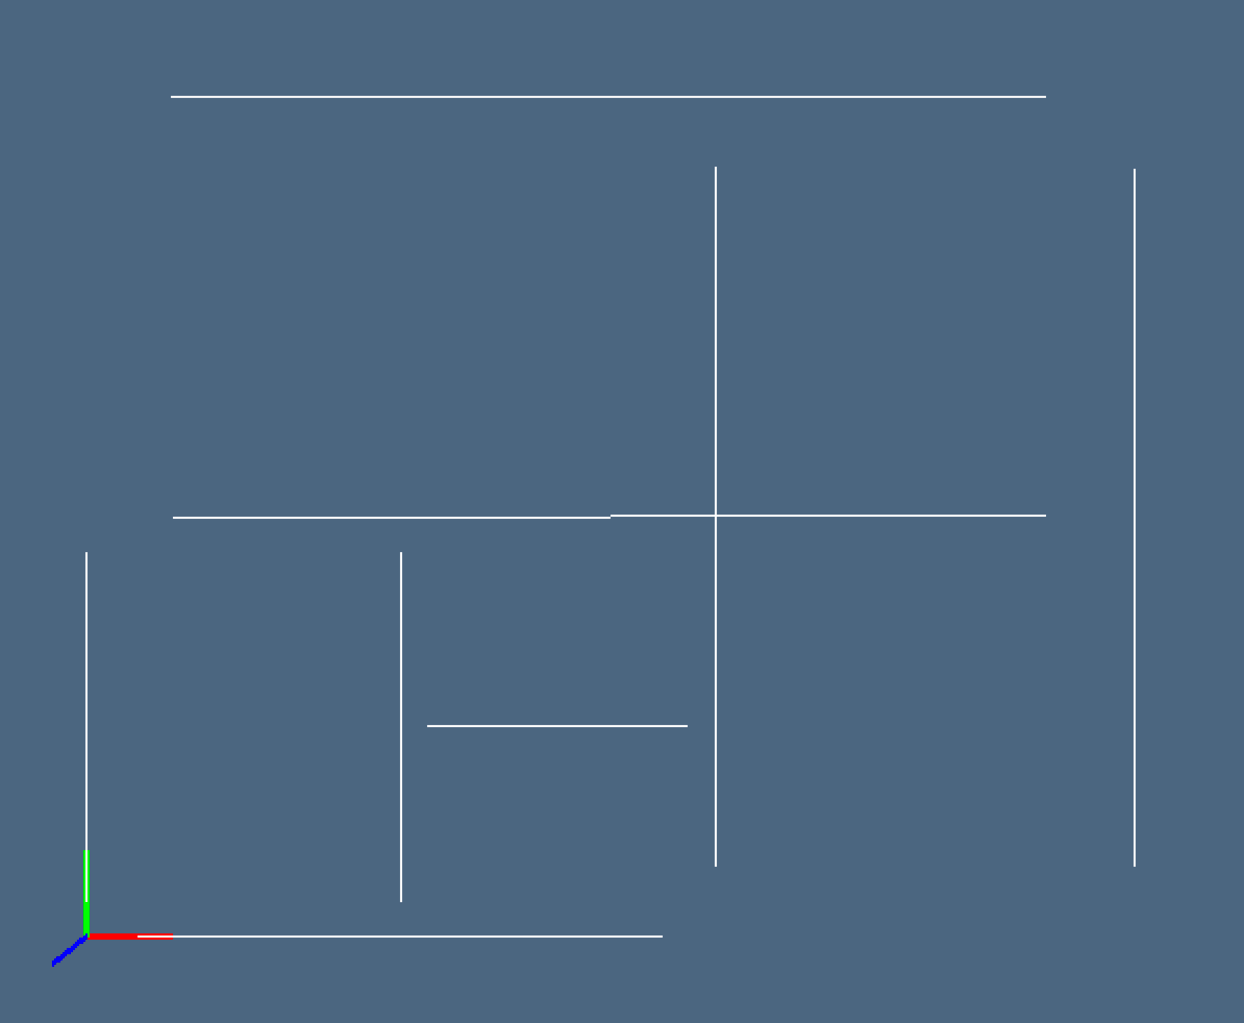
\includegraphics[height=0.25\linewidth,width=0.325\linewidth]{images/ortho1} 
   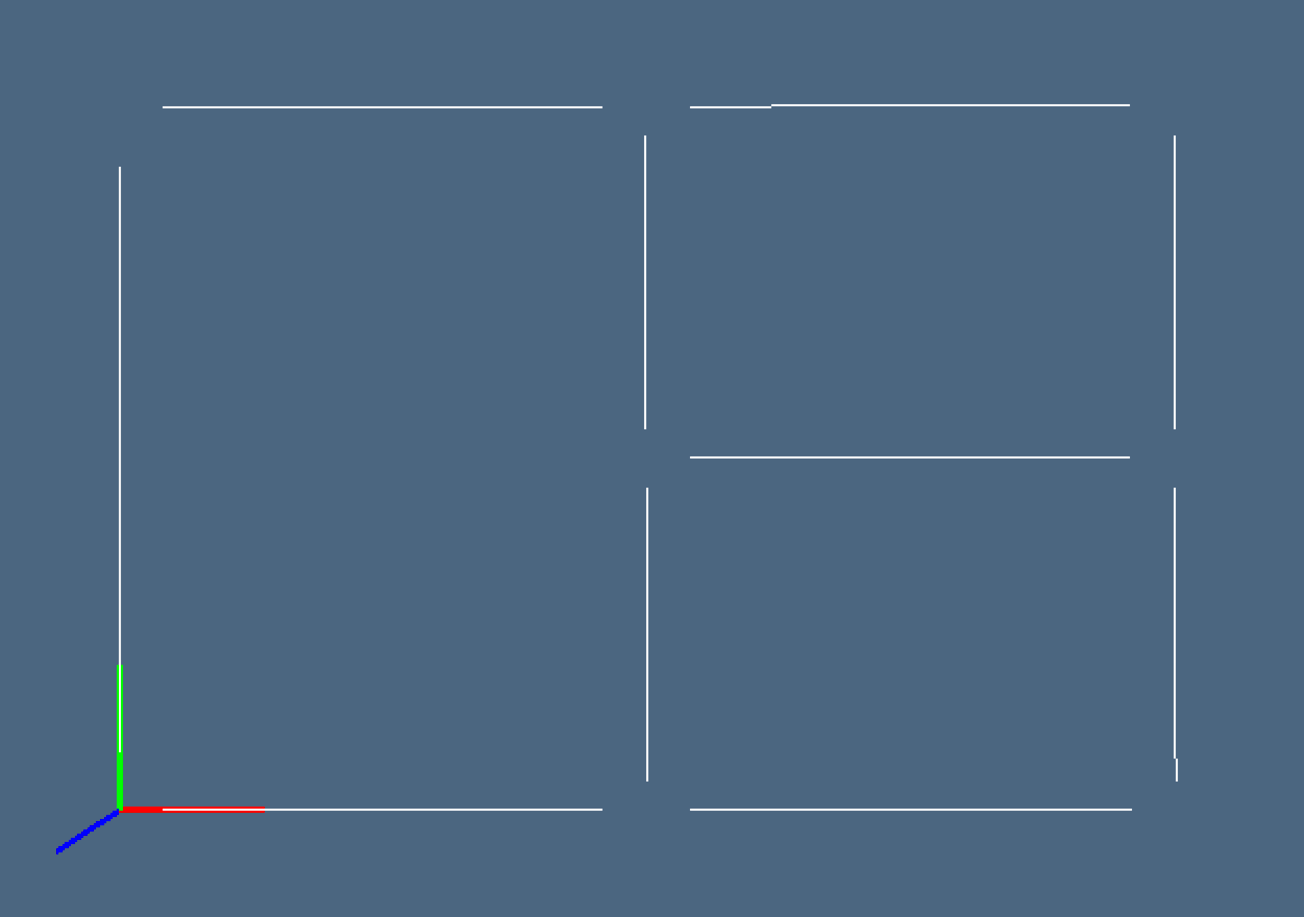
\includegraphics[height=0.25\linewidth,width=0.325\linewidth]{images/ortho2} 
   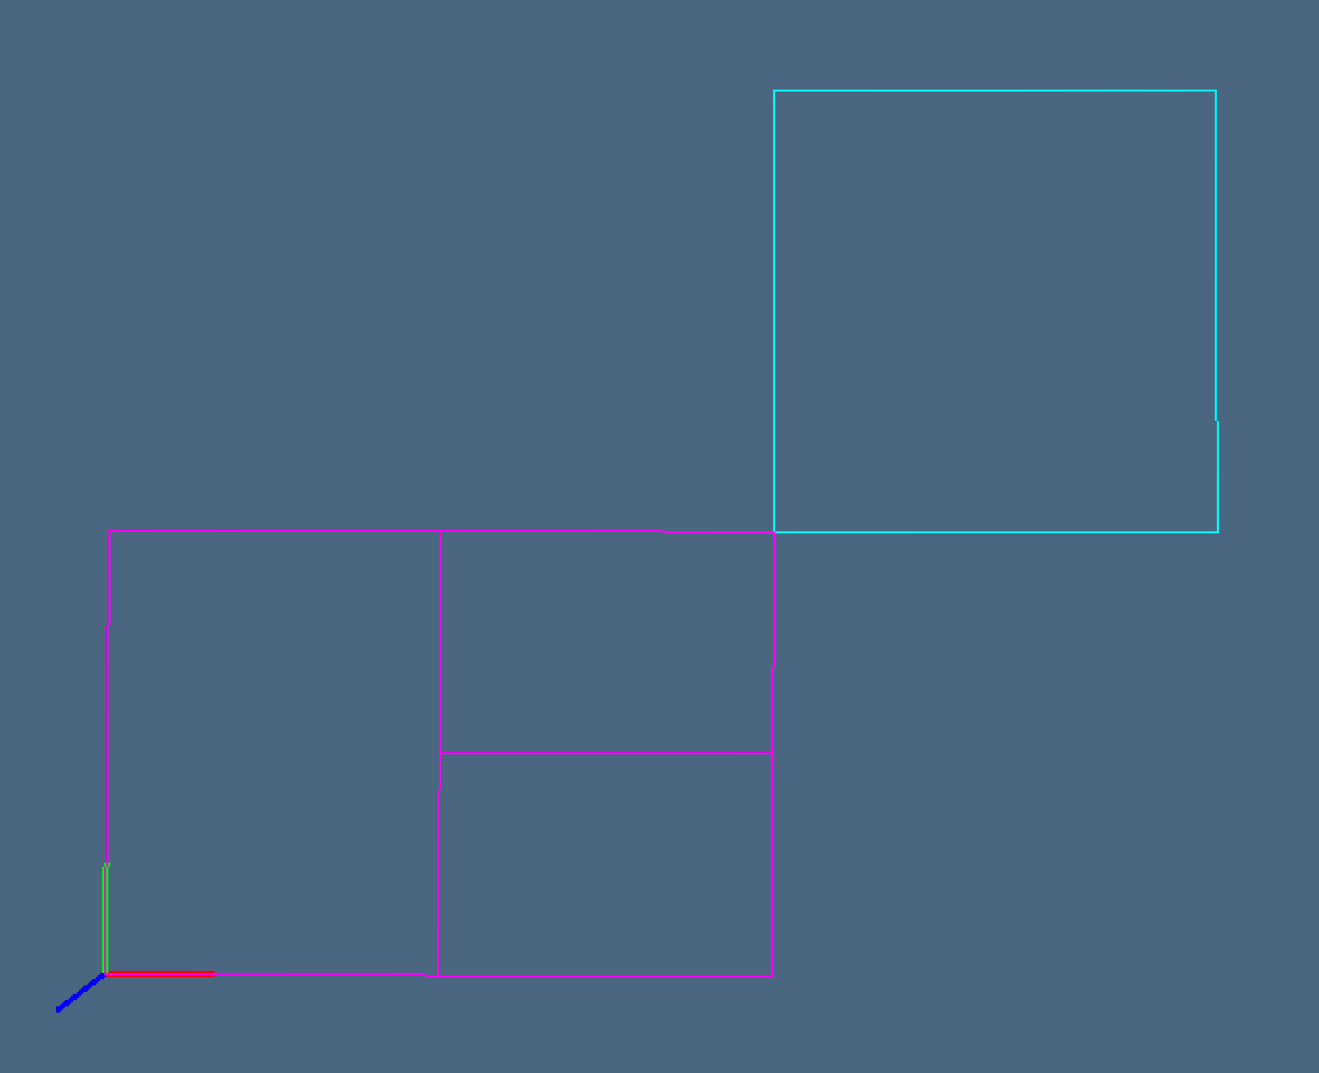
\includegraphics[height=0.25\linewidth,width=0.325\linewidth]{images/ortho3} 
   \caption{Splitting of orthogonal lines: (a) exploded input; (a) exploded output; (c) biconnected components.}
   \label{fig:ortho}
\end{figure}



\paragraph{Random coloring of the generated 1-complex LAR}
%-------------------------------------------------------------------------------
@O test/py/inters/test06.py
@{""" Random coloring of the generated 1-complex """
from larlib import *

lines = randomLines(800,0.2)
VIEW(STRUCT(AA(POLYLINE)(lines)))

V,EV = lines2lar(lines)
colors = [CYAN, MAGENTA, WHITE, RED, YELLOW, GRAY, GREEN, ORANGE, BLACK, BLUE, PURPLE, BROWN]
sets = [COLOR(colors[k%12])(POLYLINE([V[e[0]],V[e[1]]])) for k,e in enumerate(EV)]

VIEW(STRUCT(sets))
@}
%-------------------------------------------------------------------------------

\begin{figure}[htbp] %  figure placement: here, top, bottom, or page
   \centering
   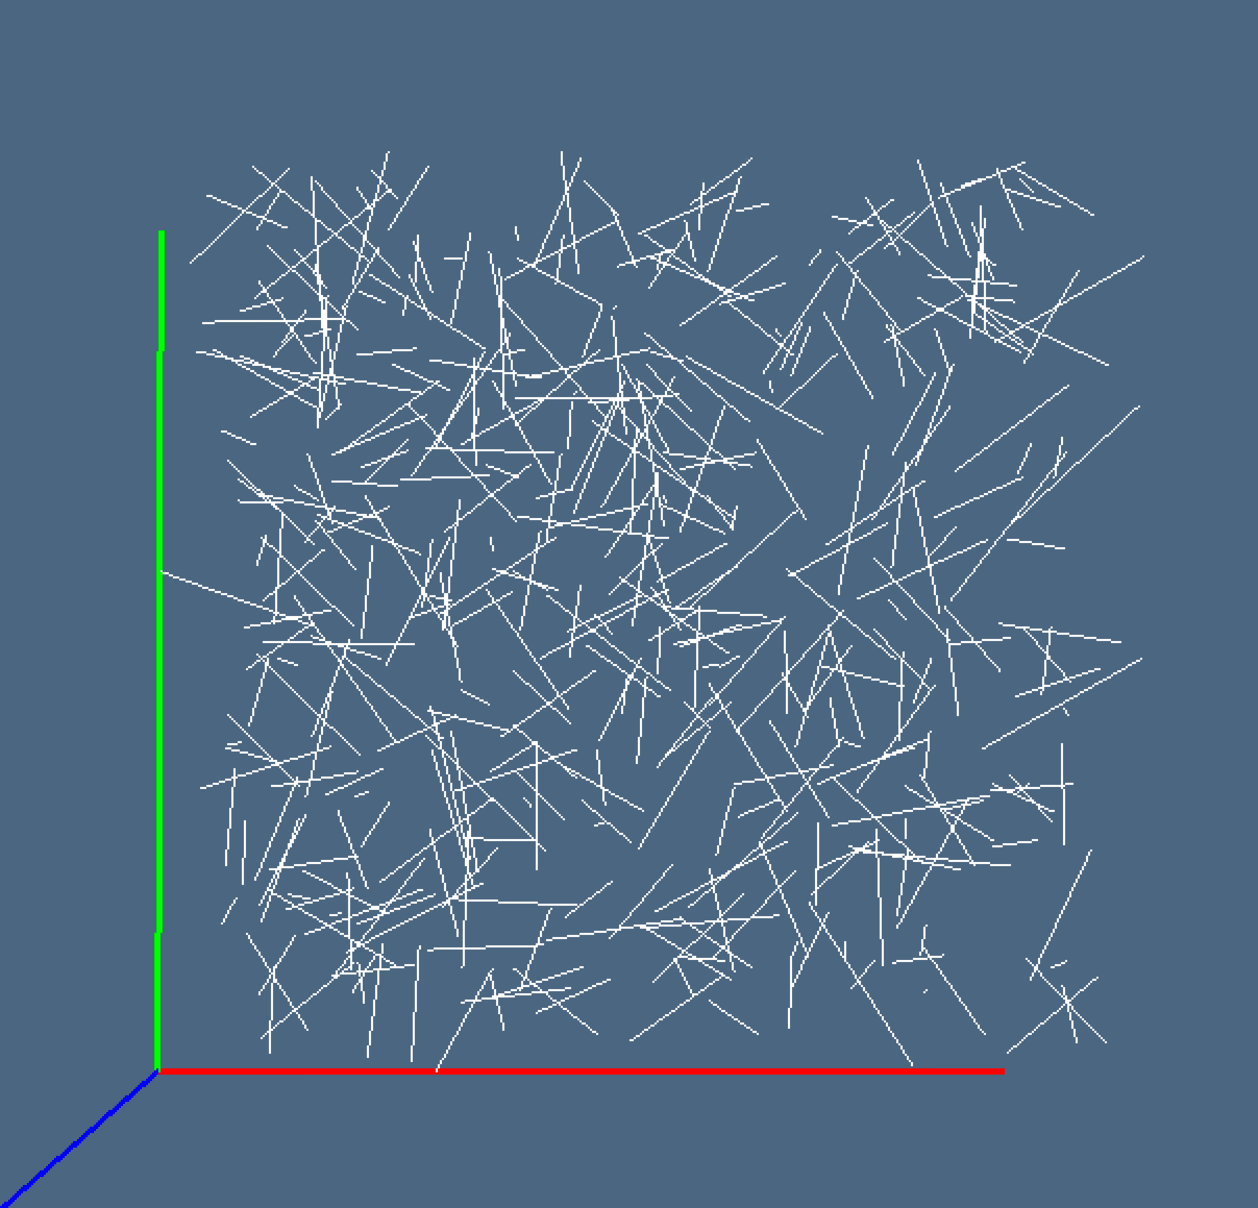
\includegraphics[width=0.49\linewidth]{images/colored1} 
   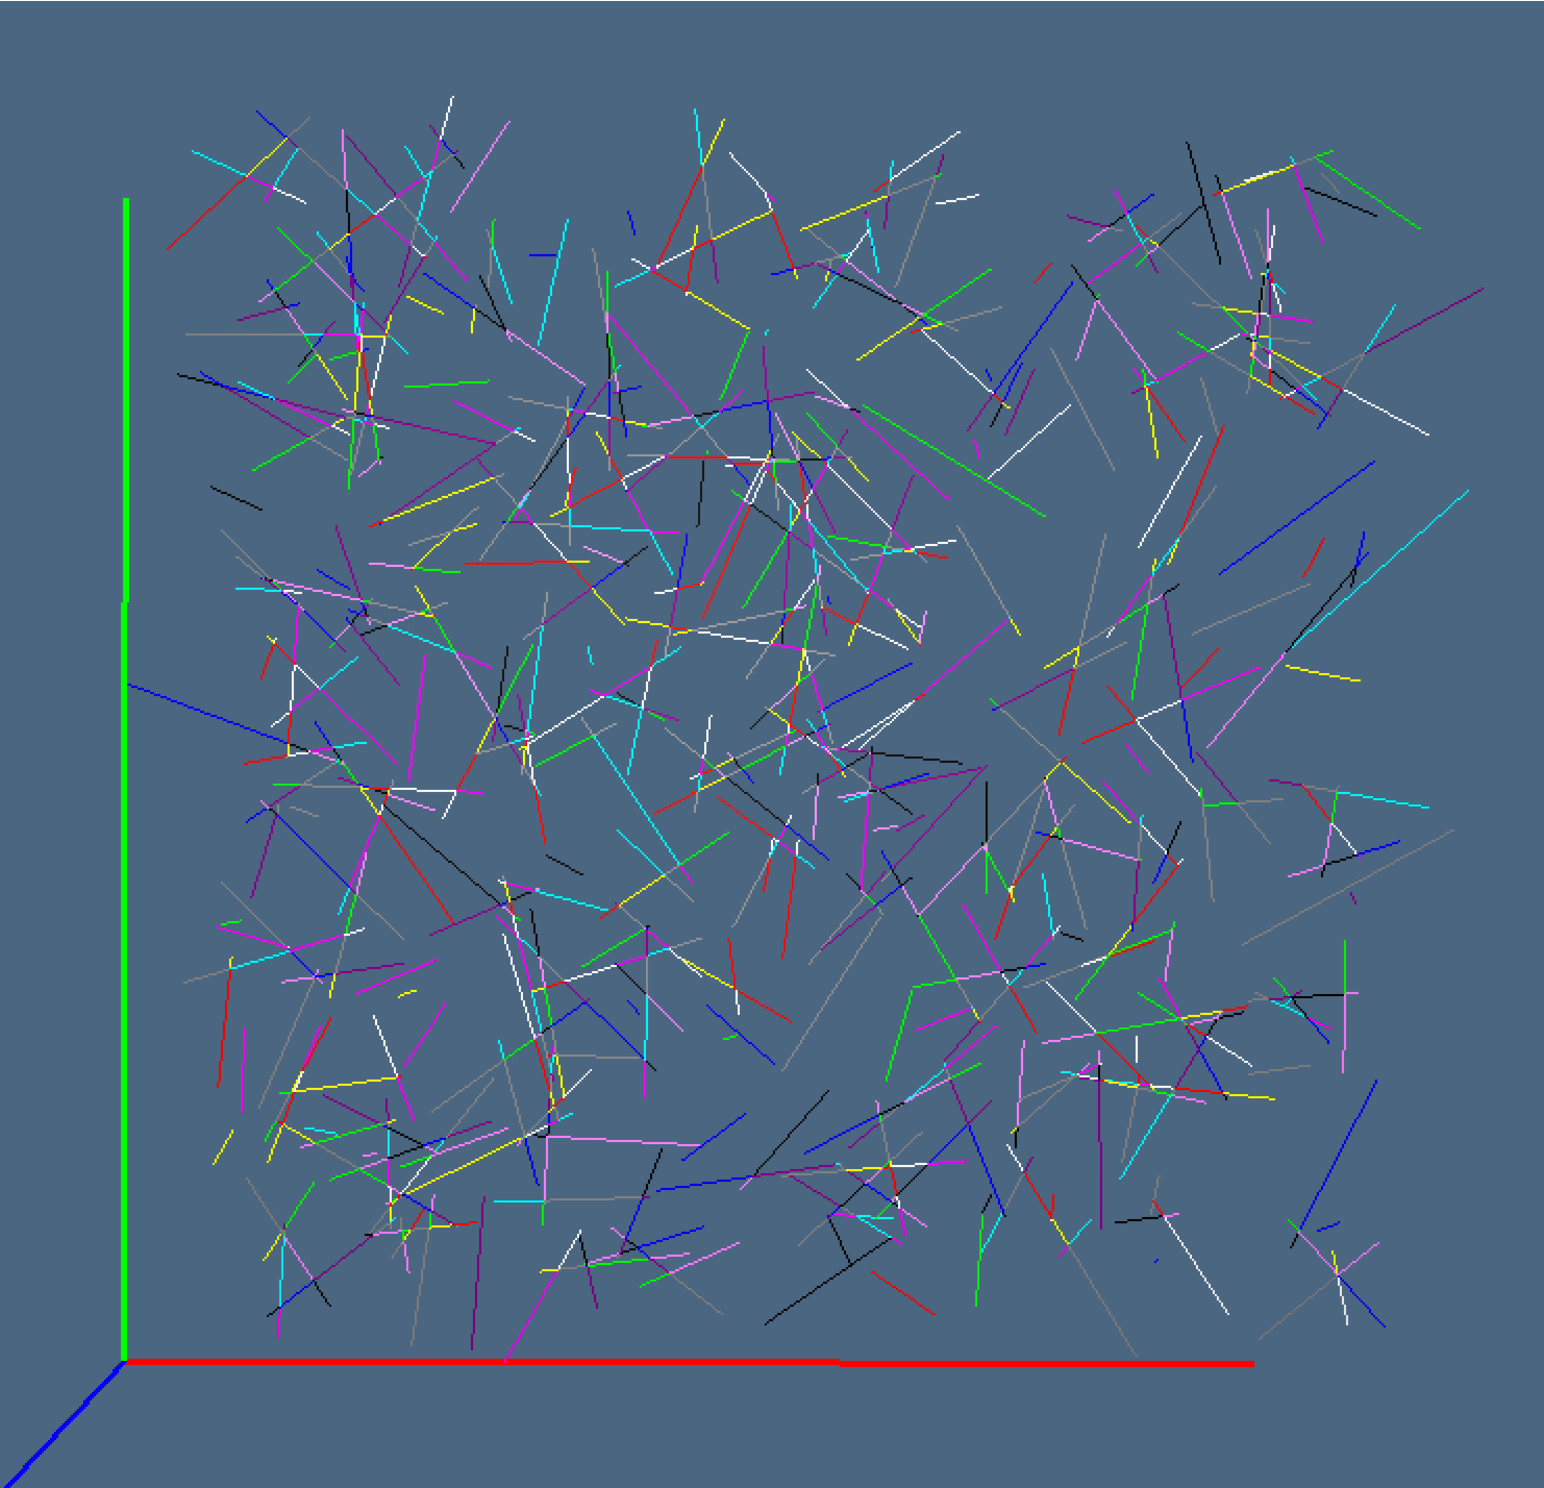
\includegraphics[width=0.49\linewidth]{images/colored2} 
   \caption{Splitting of intersecting lines: (a) random input; (a) splitted and colored LAR output.}
   \label{fig:ortho}
\end{figure}



\begin{figure}[htbp] %  figure placement: here, top, bottom, or page
   \centering
   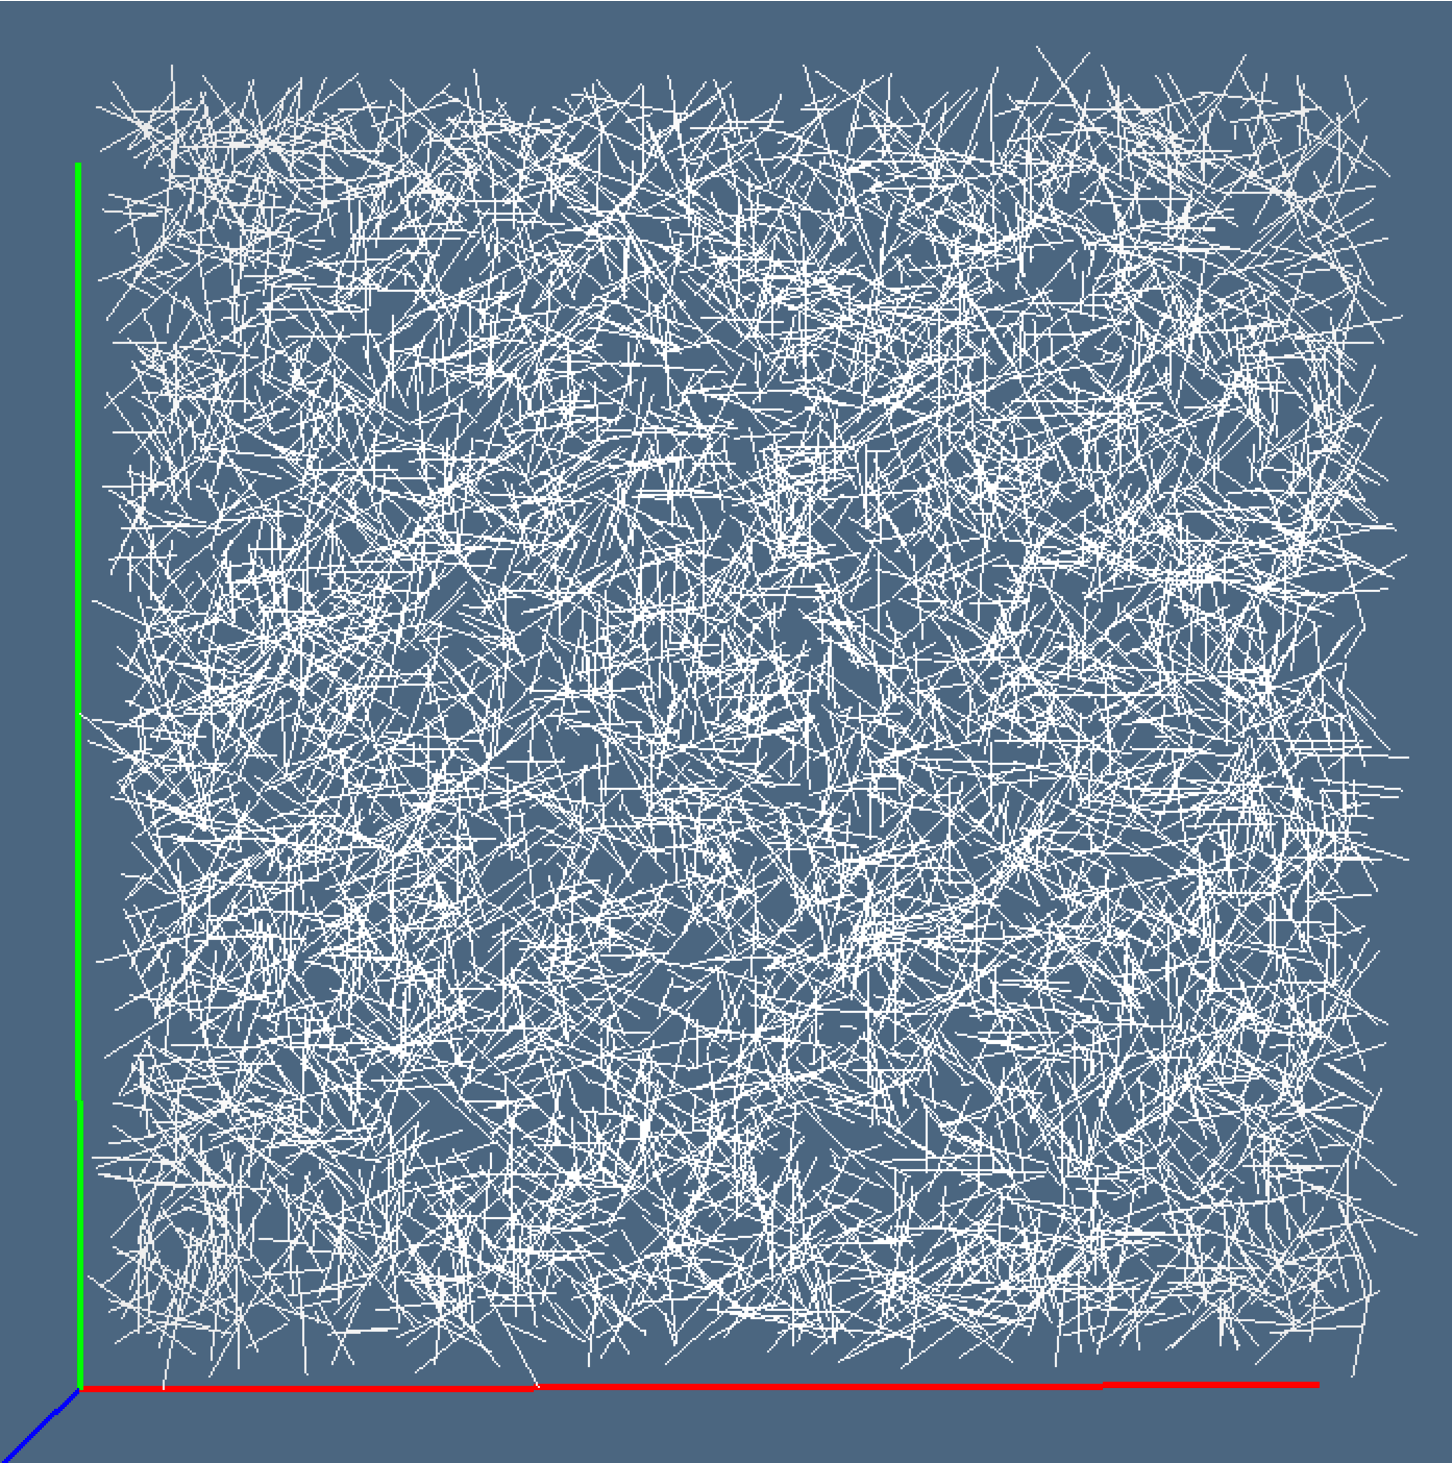
\includegraphics[height=0.49\linewidth,width=0.49\linewidth]{images/lineintersect1} 
   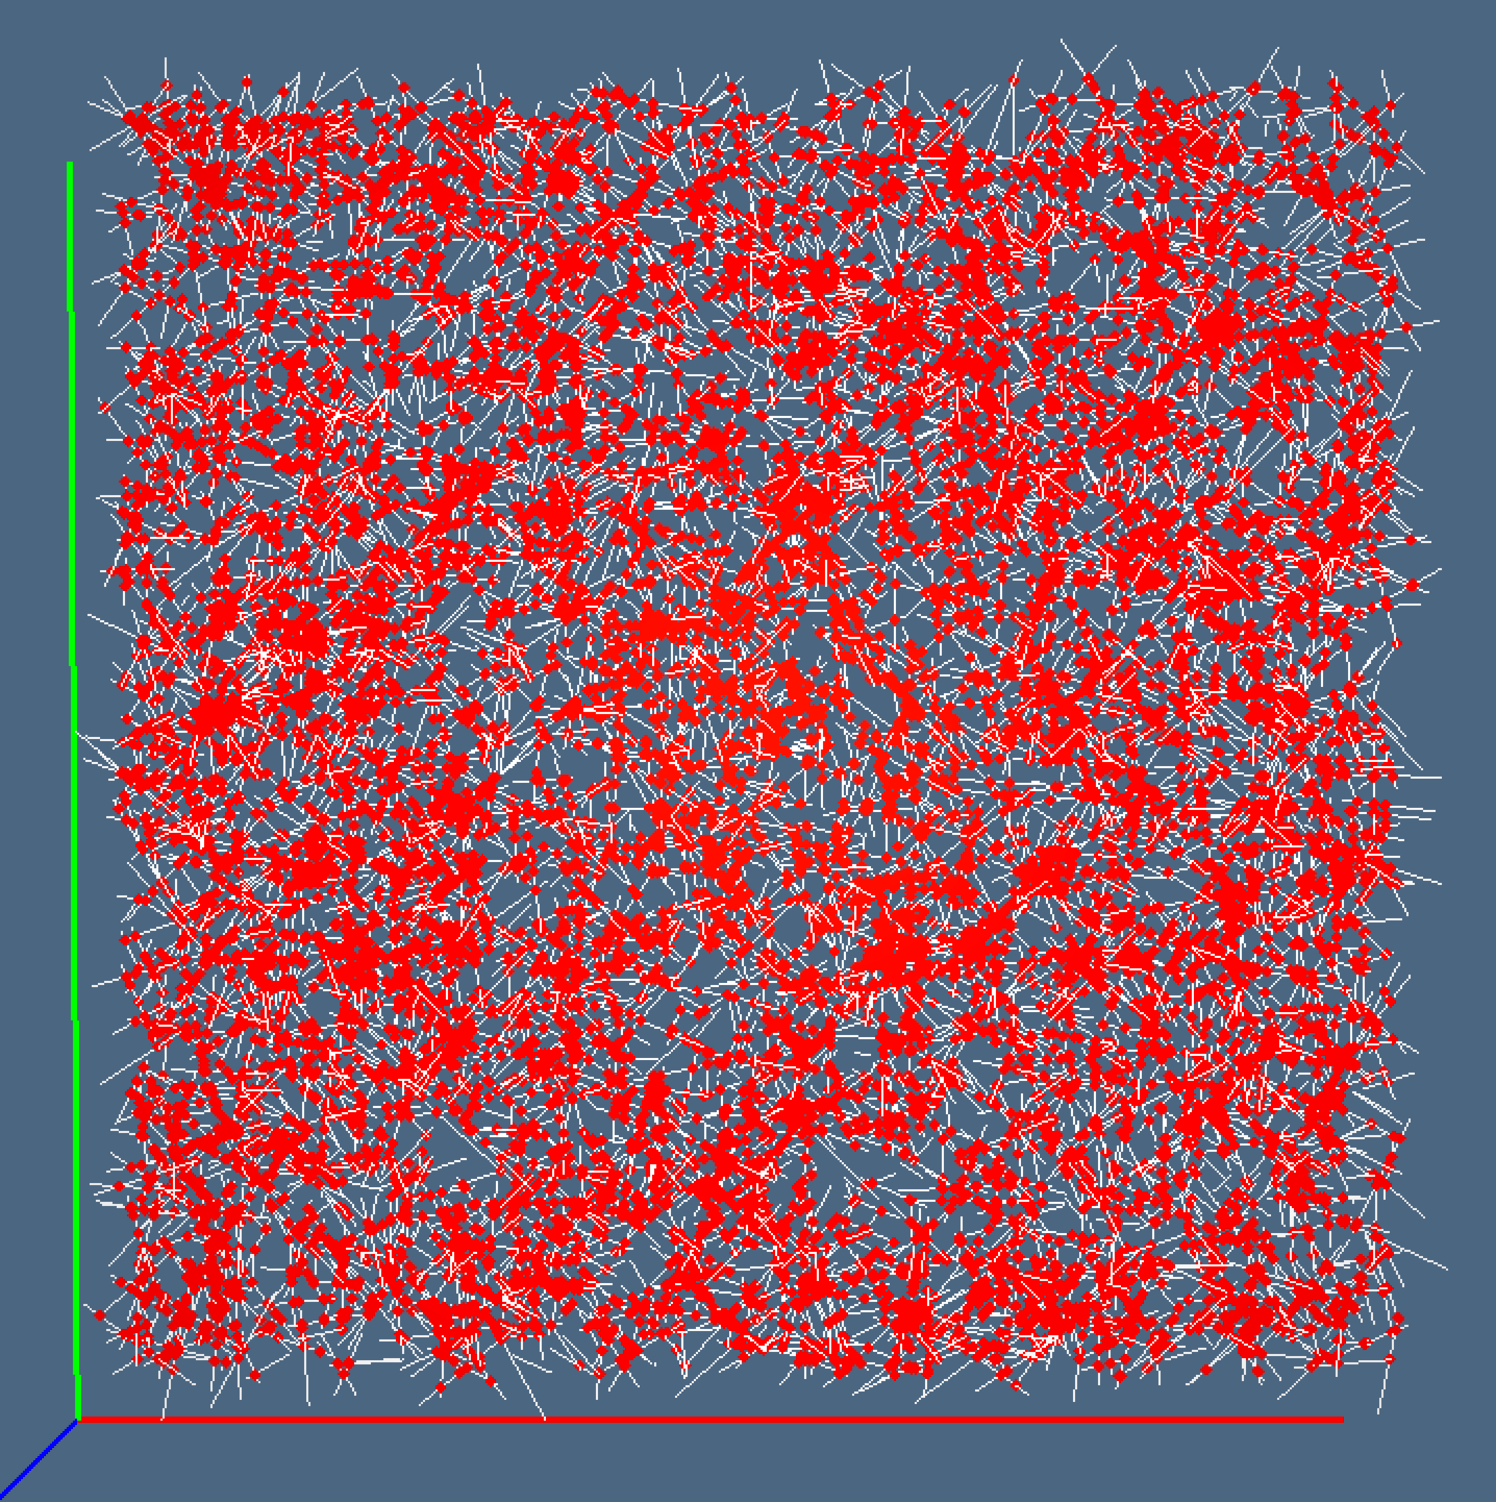
\includegraphics[height=0.49\linewidth,width=0.49\linewidth]{images/lineintersect2} 
   \caption{The intersection of 5000 random lines in the unit interval, with \texttt{scaling} parameter equal to \texttt{0.1}}
   \label{fig:example}
\end{figure}


    

\paragraph{Biconnected components from orthogonal LAR model}
%-------------------------------------------------------------------------------
@O test/py/inters/test07.py
@{""" Biconnected components from orthogonal LAR model """
from larlib import *
colors = [CYAN, MAGENTA, WHITE, RED, YELLOW, GREEN, ORANGE, BLACK, BLUE, PURPLE]

@< Orthogonal example @>
model = V,EV
V,EVs = biconnectedComponent(model)
HPCs = [STRUCT(MKPOLS((V,EV))) for EV in EVs]

sets = [COLOR(colors[k%10])(hpc) for k,hpc in enumerate(HPCs)]
VIEW(STRUCT(sets))
VIEW(STRUCT(MKPOLS((V,CAT(EVs)))))

#V,EV = larRemoveVertices(V,CAT(EVs))
@}
%-------------------------------------------------------------------------------


\paragraph{2-complex from orthogonal line segments}
%-------------------------------------------------------------------------------
@O test/py/inters/test08.py
@{""" 2-complex from orthogonal line segments """
from larlib import *
colors = [CYAN, MAGENTA, WHITE, RED, YELLOW, GREEN, ORANGE, BLACK, BLUE, PURPLE]

@< Orthogonal example @>
model = V,EV
V,EVs = biconnectedComponent(model)
HPCs = [STRUCT(MKPOLS((V,EV))) for EV in EVs]

sets = [COLOR(colors[k%10])(hpc) for k,hpc in enumerate(HPCs)]
VIEW(STRUCT(sets))

EV = sorted(CAT(EVs))
VIEW(STRUCT(MKPOLS((V,EV))))

V,FV,EV = facesFromComps((V,EV))

areas = surfIntegration((V,FV,EV))
boundaryArea = max(areas)
FV = [FV[f] for f,area in enumerate(areas) if area!=boundaryArea]
VIEW(EXPLODE(1.2,1.2,1)(MKPOLS((V,FV+EV)) + AA(MK)(V)))
@}
%-------------------------------------------------------------------------------


\begin{figure}[htbp] %  figure placement: here, top, bottom, or page
   \centering
   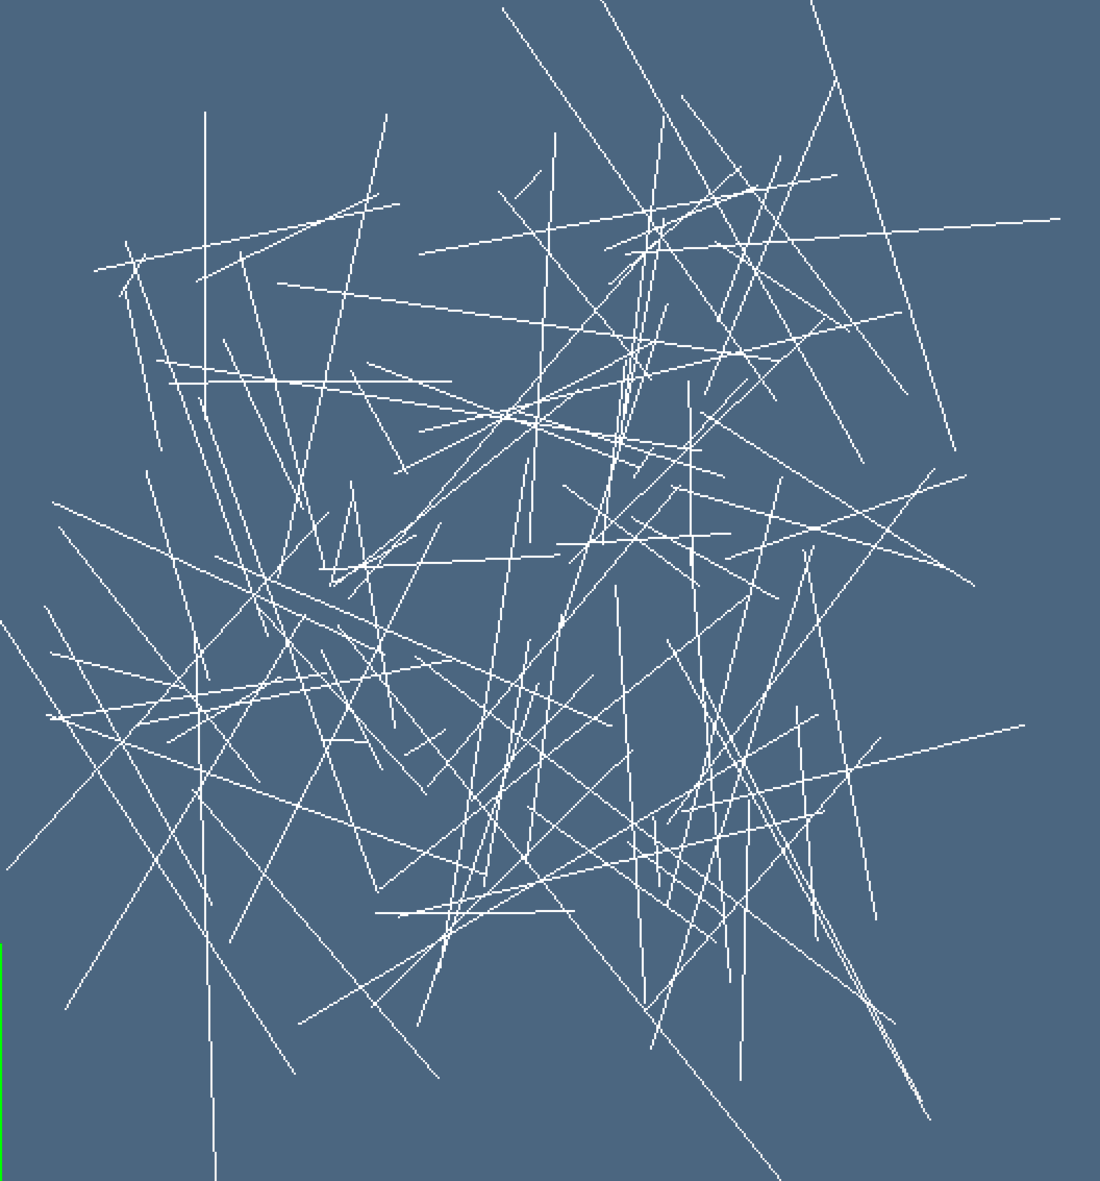
\includegraphics[height=0.325\linewidth,width=0.325\linewidth]{images/random2d0} 
   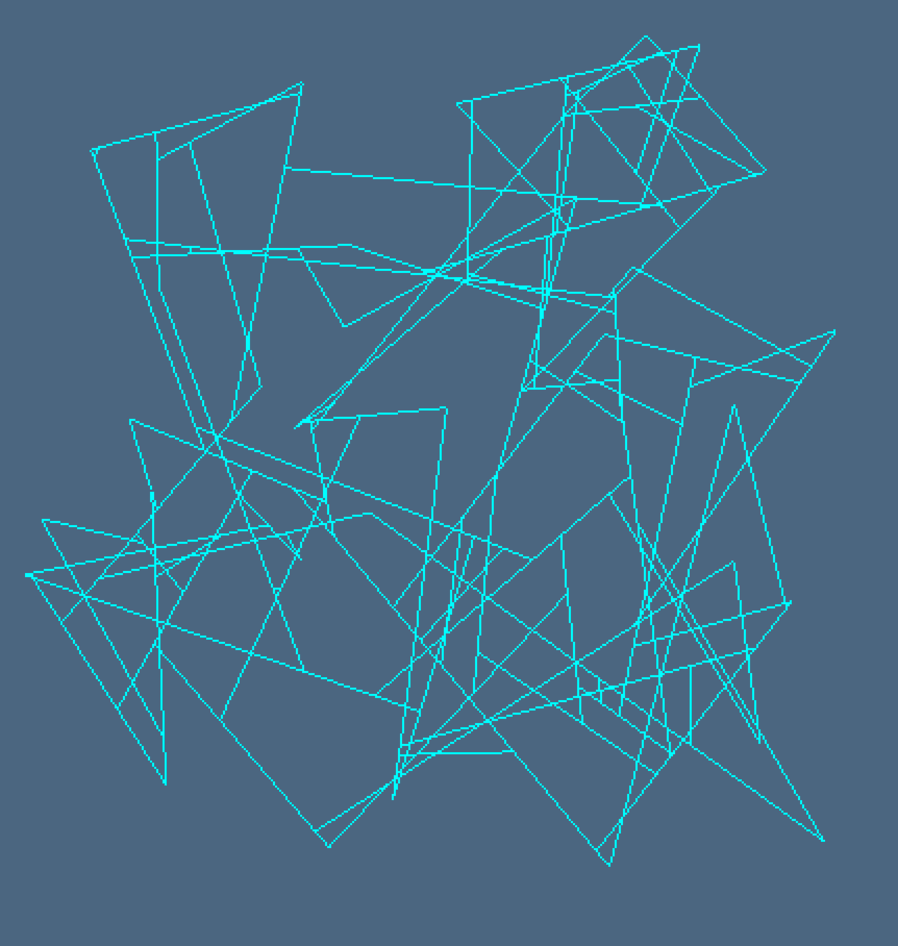
\includegraphics[height=0.325\linewidth,width=0.325\linewidth]{images/random2d1} 
   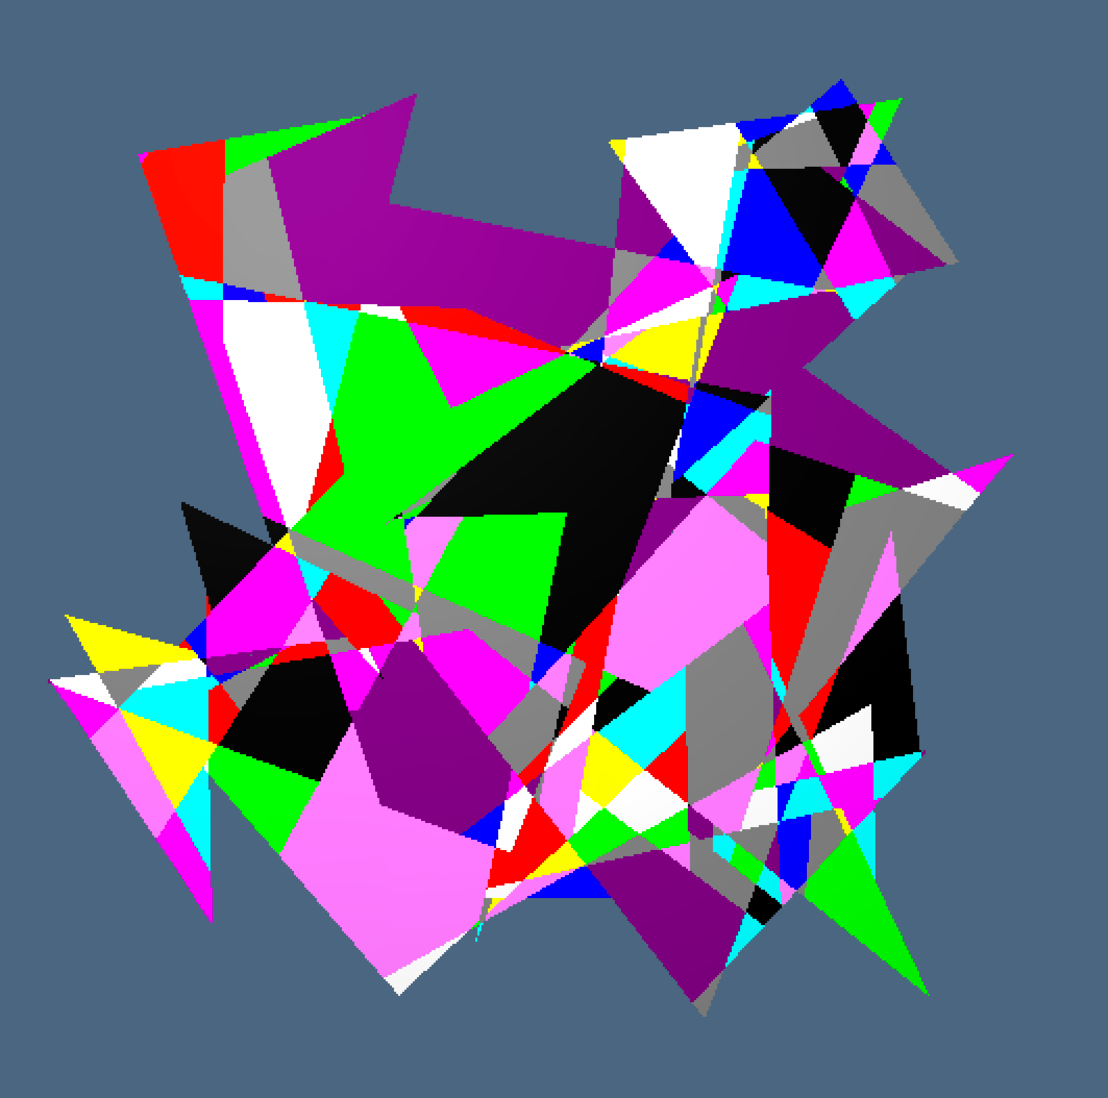
\includegraphics[height=0.325\linewidth,width=0.325\linewidth]{images/random2d2} 

   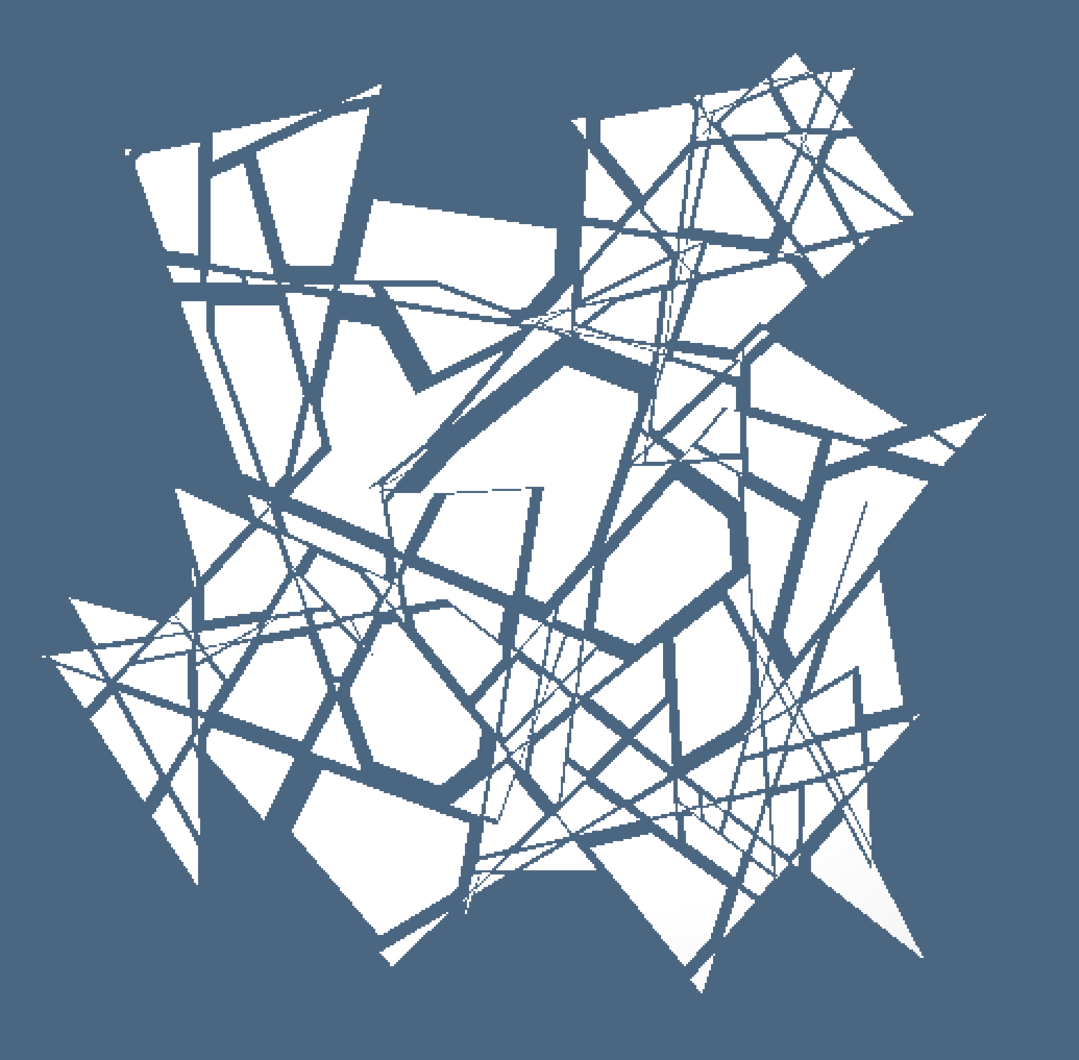
\includegraphics[height=0.325\linewidth,width=0.325\linewidth]{images/random2d3} 
   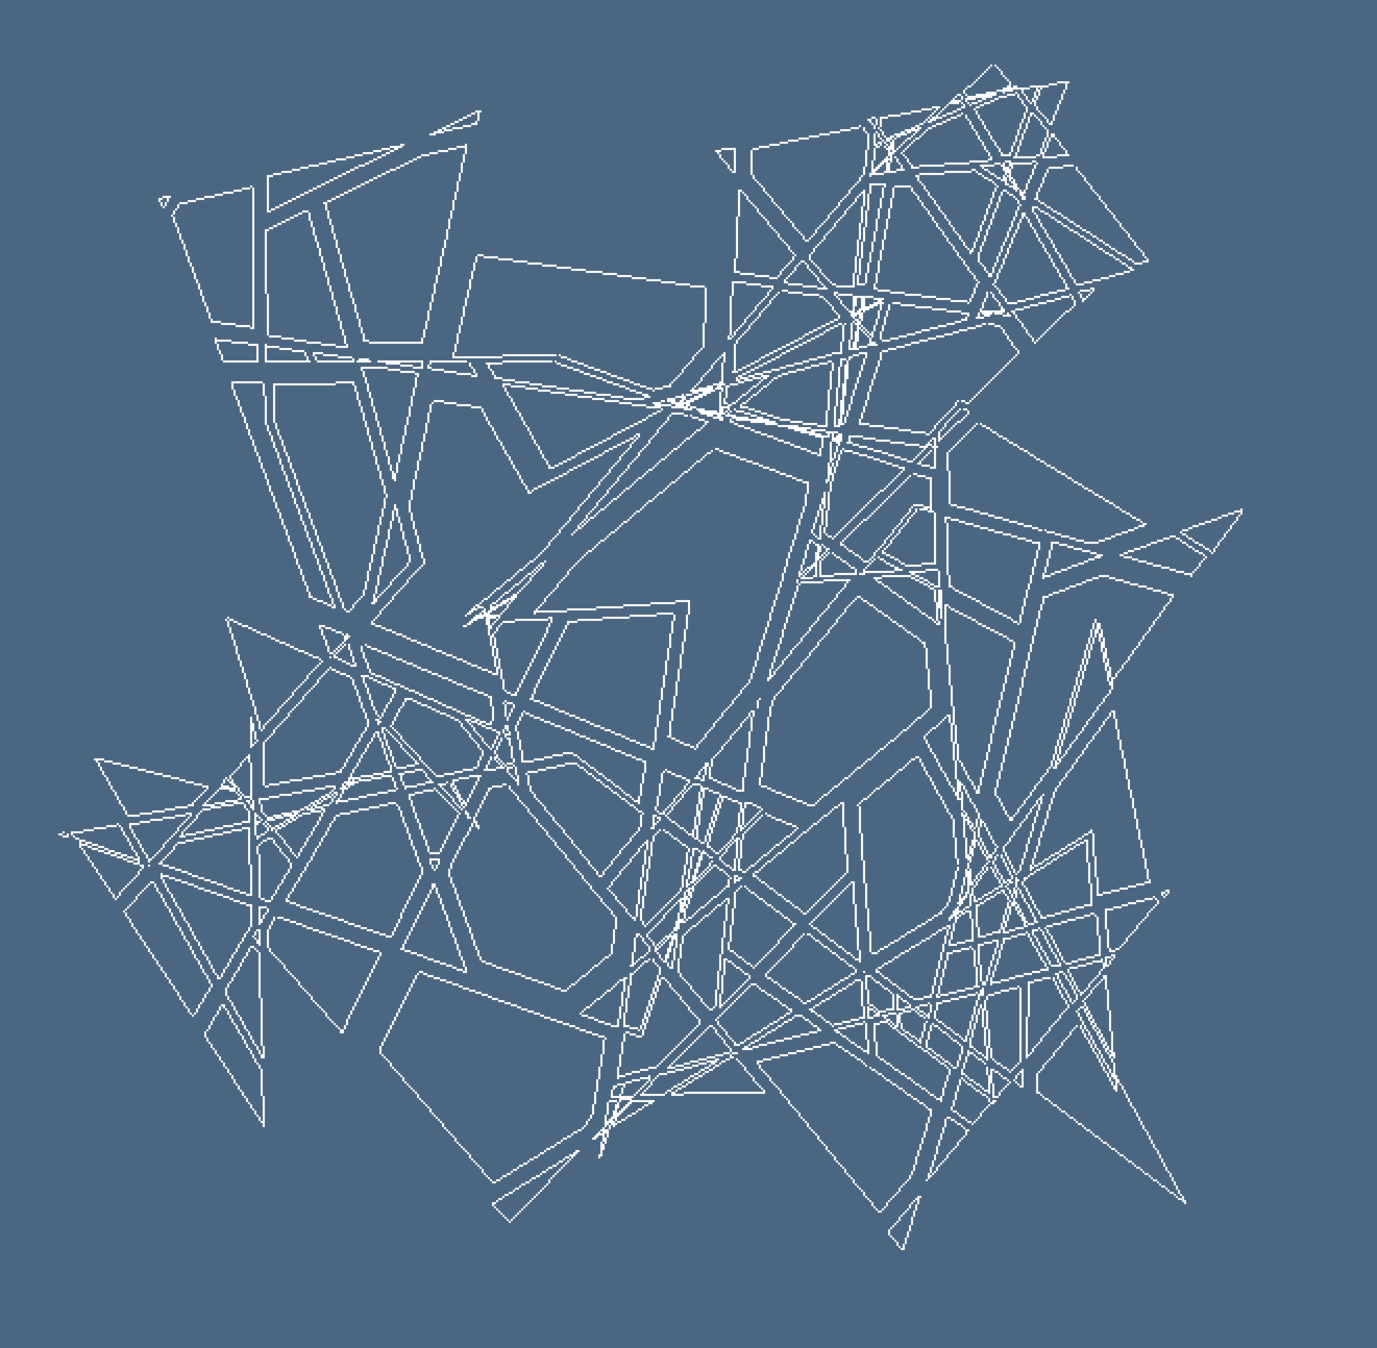
\includegraphics[height=0.325\linewidth,width=0.325\linewidth]{images/random2d4} 
   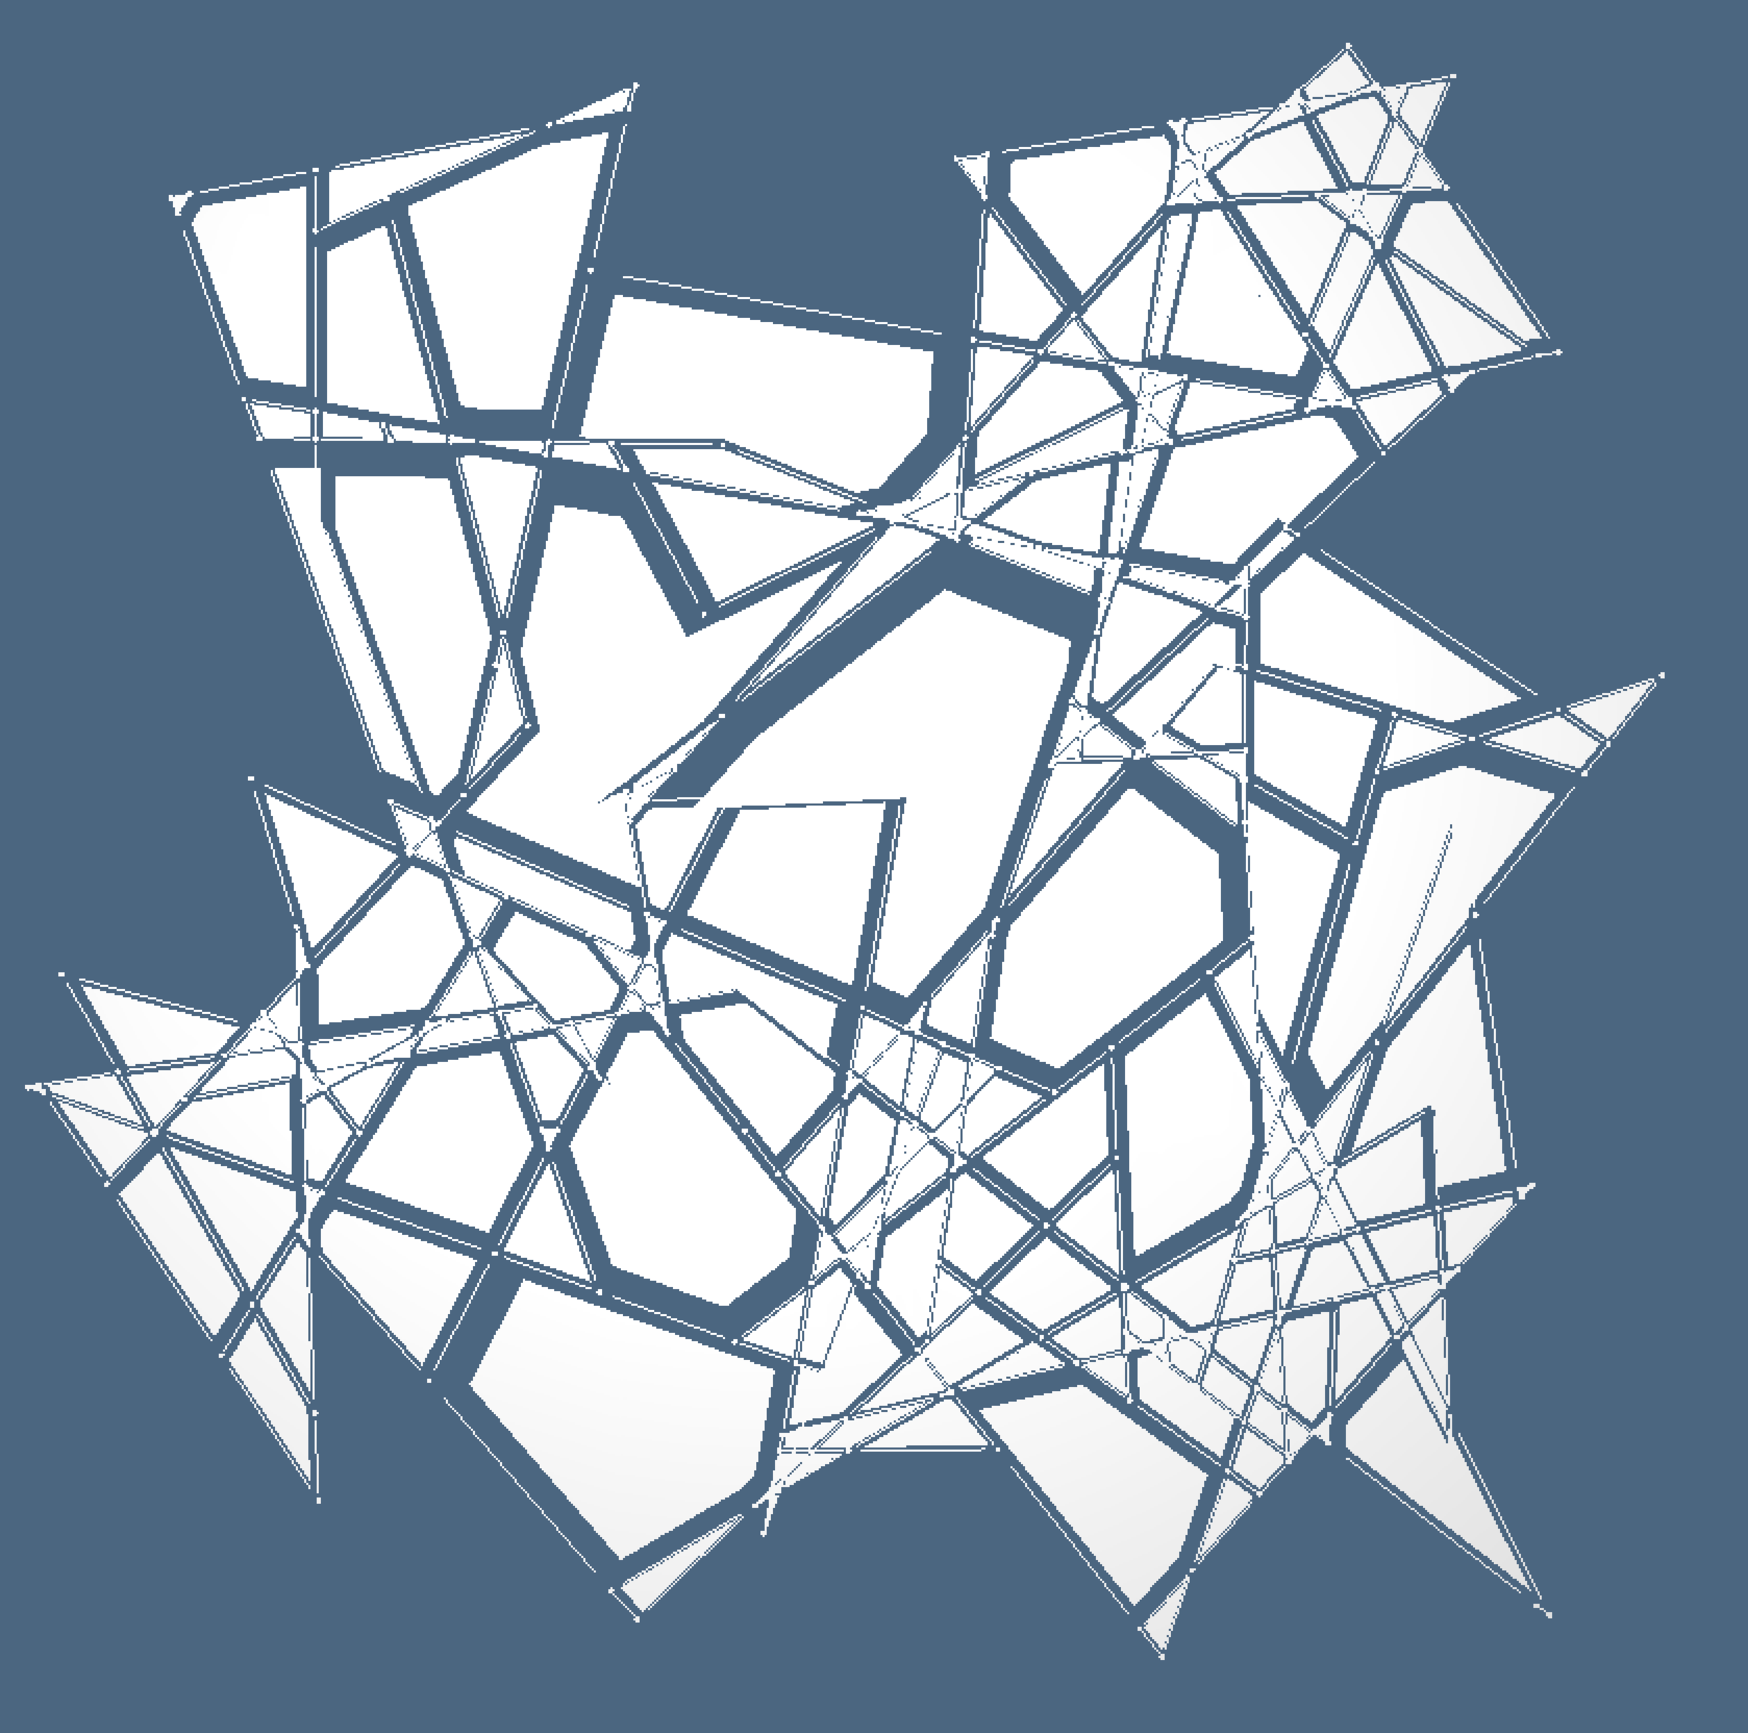
\includegraphics[height=0.325\linewidth,width=0.325\linewidth]{images/random2d5} 
   \caption{\texttt{LAR} complex generation random lines. (a) the input random lines; (b) maximal biconnected graph extracted from the 1D LAR of intersected lines; (c) 2D cells of such \emph{regularized} 2-complex; (d) 2-cells, drawn exploded; (e) boundaries of 2D cells; (f) regularized cellular 2-complex extracted from lines.}
   \label{fig:ortho}
\end{figure}

\paragraph{Biconnected components from random LAR model}
%-------------------------------------------------------------------------------
@O test/py/inters/test09.py
@{""" Biconnected components from orthogonal LAR model """
from larlib import *
colors = [CYAN, MAGENTA, YELLOW, RED, GREEN, ORANGE, PURPLE, WHITE, BLACK, BLUE]

lines = randomLines(100,.8)
V,EV = lines2lar(lines)
model = V,EV
VIEW(STRUCT(AA(POLYLINE)(lines)))

V,EVs = biconnectedComponent(model)
HPCs = [STRUCT(MKPOLS((V,EV))) for EV in EVs]
sets = [COLOR(colors[k%10])(hpc) for k,hpc in enumerate(HPCs)]
VIEW(STRUCT(sets))

EV = CAT(EVs)
V,EV = larRemoveVertices(V,EV)
V,FV,EV = facesFromComps((V,EV))
areas = surfIntegration((V,FV,EV))
boundaryArea = max(areas)
FV = [FV[f] for f,area in enumerate(areas) if area!=boundaryArea]

polylines = [[V[v] for v in face+[face[0]]] for face in FV]
VIEW(EXPLODE(1.2,1.2,1)(MKPOLS((V,EV)) + AA(MK)(V) + AA(FAN)(polylines) ))

colors = [CYAN, MAGENTA, WHITE, RED, YELLOW, GRAY, GREEN, ORANGE, BLACK, BLUE, PURPLE, BROWN]
sets = [COLOR(colors[k%12])(FAN(pol)) for k,pol in enumerate(polylines)]
VIEW(STRUCT(sets))


VIEW(EXPLODE(1.2,1.2,1)((AA(FAN)(polylines))))
VIEW(EXPLODE(1.2,1.2,1)((AA(POLYLINE)(polylines))))

VV = AA(LIST)(range(len(V)))
submodel = STRUCT(MKPOLS((V,EV)))
VIEW(larModelNumbering(1,1,1)(V,[VV,EV],submodel,0.1))
@}
%-------------------------------------------------------------------------------



\begin{figure}[htbp] %  figure placement: here, top, bottom, or page
   \centering
   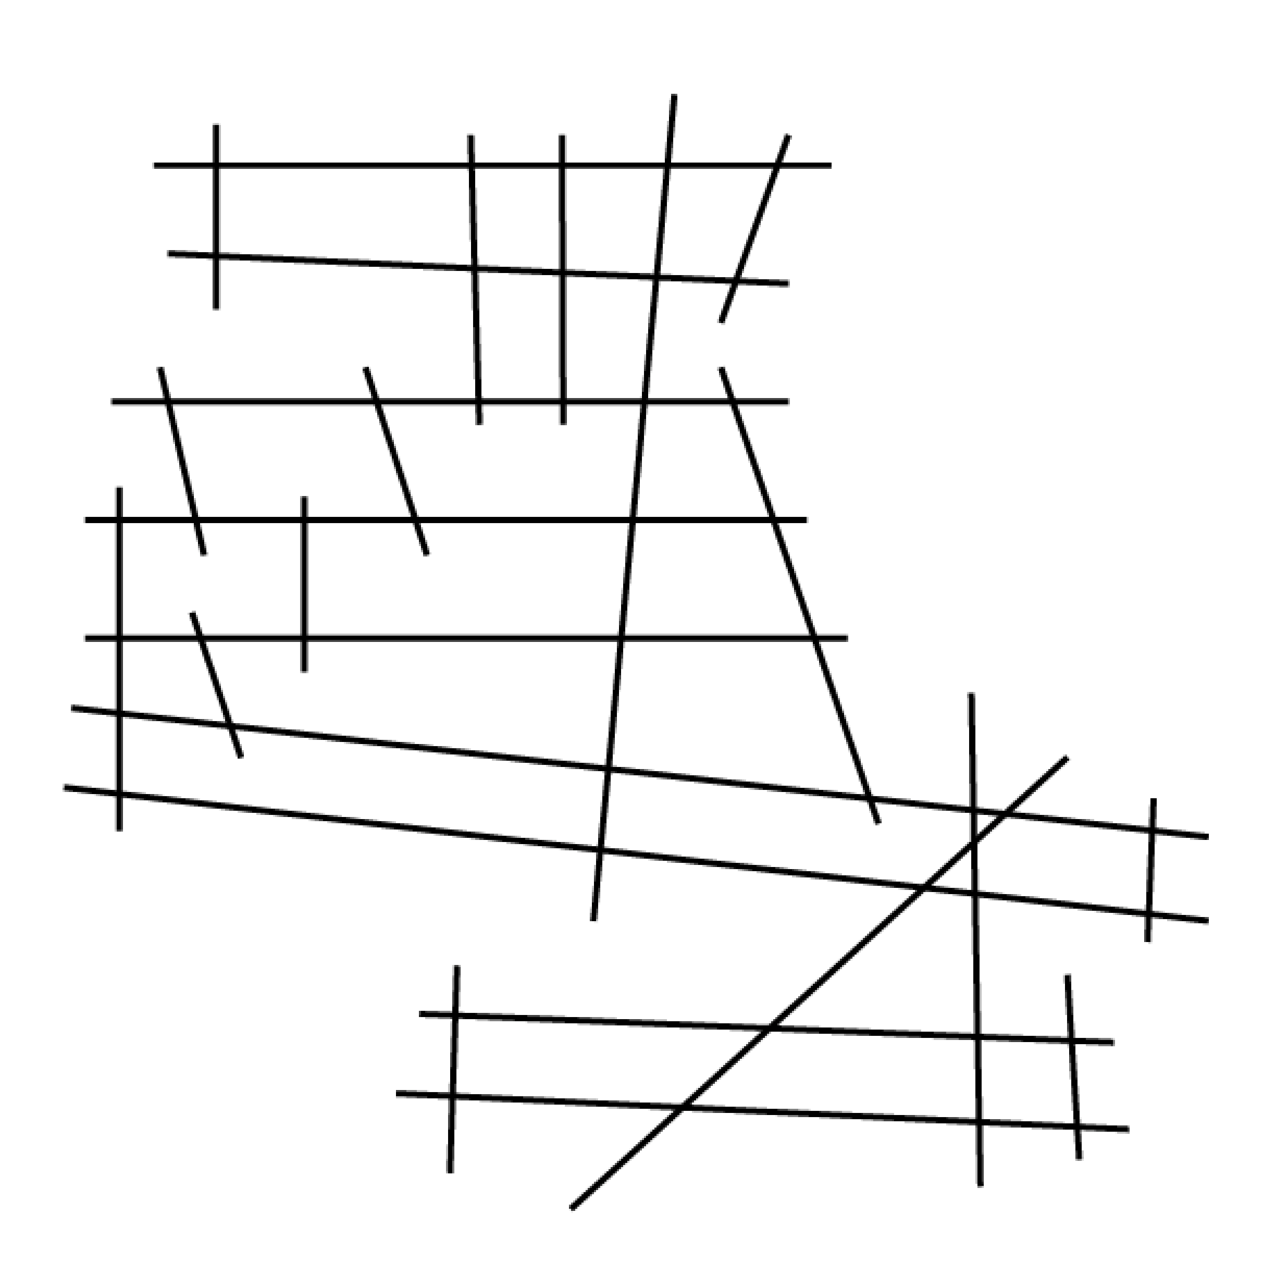
\includegraphics[height=0.325\linewidth,width=0.325\linewidth]{images/illustrator1} 
   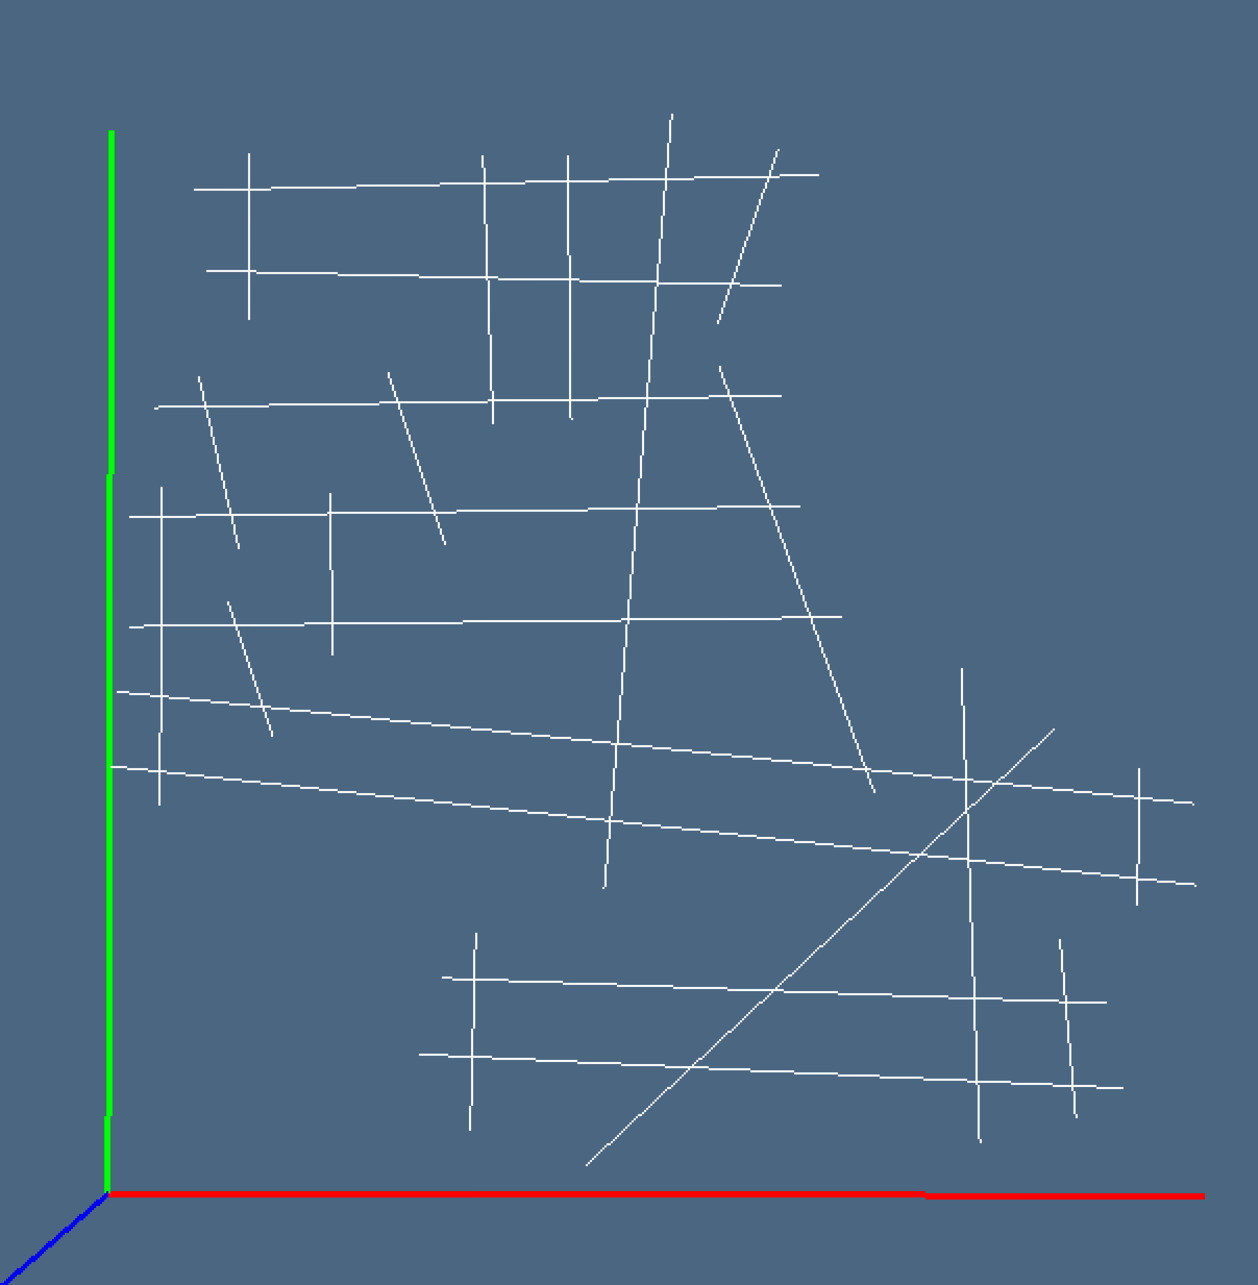
\includegraphics[height=0.325\linewidth,width=0.325\linewidth]{images/illustrator2} 
   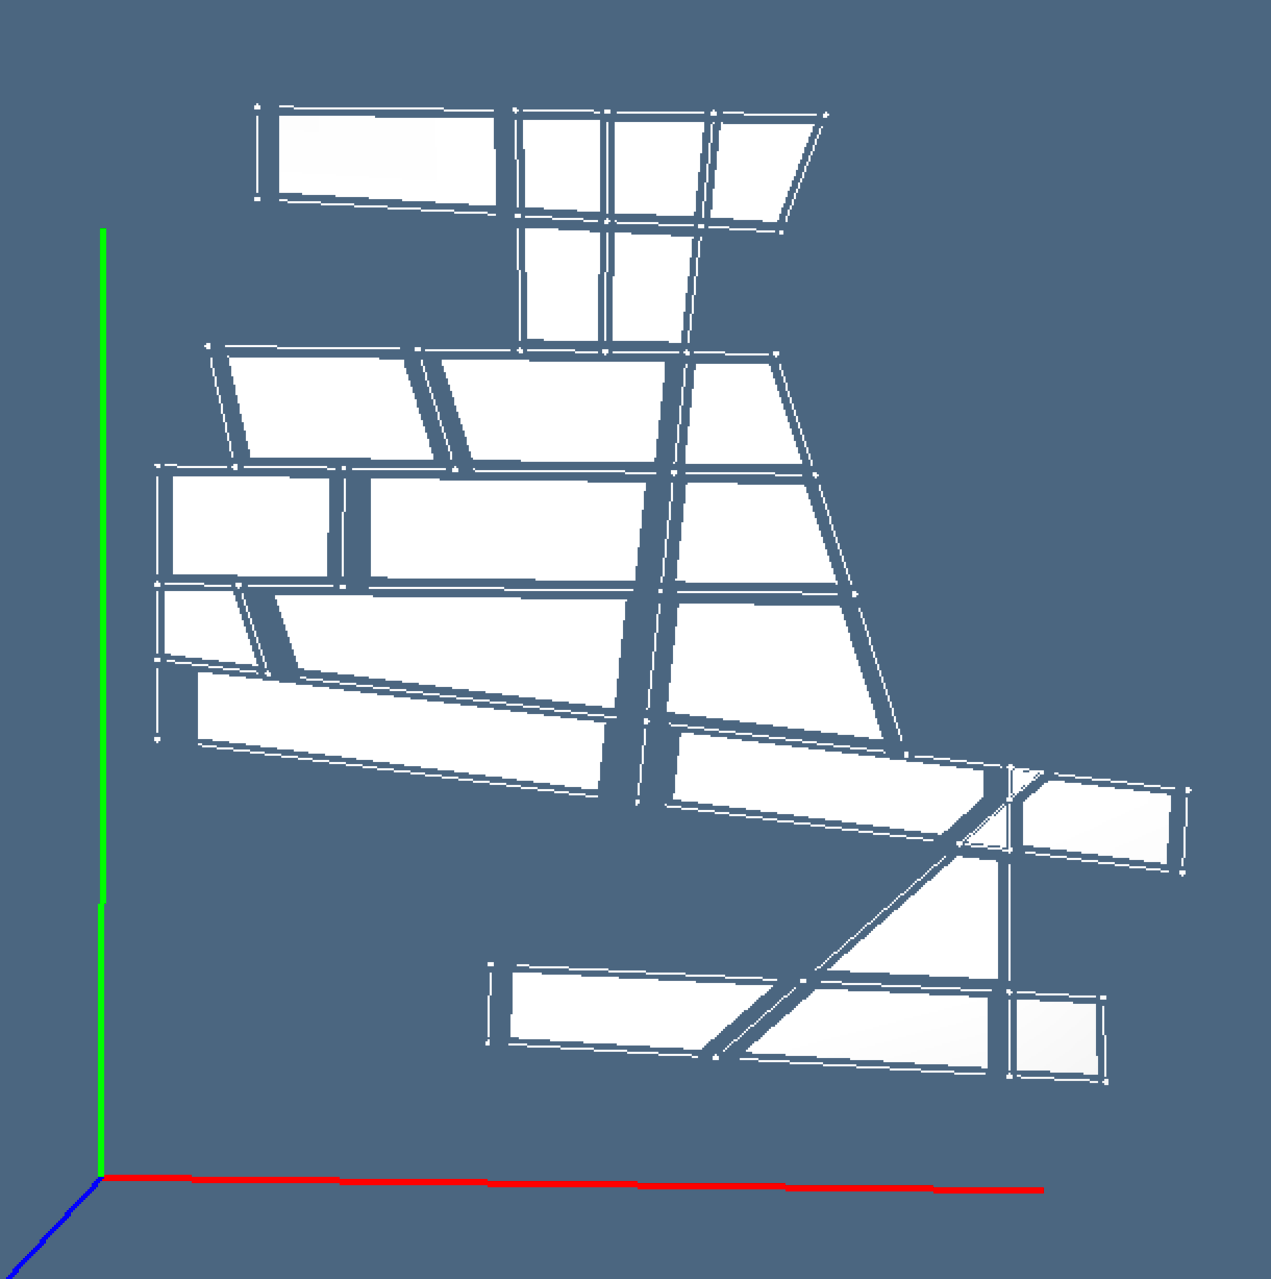
\includegraphics[height=0.325\linewidth,width=0.325\linewidth]{images/illustrator3} 
   \caption{\texttt{LAR} complex generation from \texttt{SVG} file. (a) the input set of lines; (b) imported in \texttt{pyplasm} environment; (c) the extracted \emph{regularized} 2-complex, drawn exploded.}
   \label{fig:ortho}
\end{figure}




\paragraph{SVG input parsing and transformation}

We postulate here that the input file \texttt{test/py/inters/test.svg} should contain only \texttt{<line>} primitives, so we skip any other content. Such primitives are parsed by matching against regular expressions, and their \texttt{x1,y1,x2,y2} attributes are extracted and stored into the \texttt{lines} variable.
An isomorphic window-viewport transformation is then performed, to transform the data within the standard unit 2D square $[0,1]^2$.
The input vertices are finally set to a fixed resolution, using the \texttt{vcode} function. 

%-------------------------------------------------------------------------------
@D SVG input parsing and transformation
@{""" SVG input parsing and transformation """
from larlib import *
import re # regular expression

def svg2lines(filename,containmentBox=[],rect2lines=True):
    stringLines = [line.strip() for line in open(filename)]   
    
    # SVG <line> primitives
    lines = [string.strip() for string in stringLines if re.match("<line ",string)!=None]   
    outLines = ""   
    for line in lines:
        searchObj = re.search( r'(<line )(.+)(" x1=")(.+)(" y1=")(.+)(" x2=")(.+)(" y2=")(.+)("/>)', line)
        if searchObj:
            outLines += "[["+searchObj.group(4)+","+searchObj.group(6)+"], ["+searchObj.group(8) +","+ searchObj.group(10) +"]],"
    if lines != []:
        lines = list(eval(outLines))
              
    # SVG <rect> primitives
    rects = [string.strip() for string in stringLines if re.match("<rect ",string)!=None]   
    outRects,searchObj = "",False 
    for rect in rects:
        searchObj = re.search( r'(<rect x=")(.+?)(" y=")(.+?)(" )(.*?)( width=")(.+?)(" height=")(.+?)("/>)', rect)
        if searchObj:
            outRects += "[["+searchObj.group(2)+","+searchObj.group(4)+"], ["+searchObj.group(8)+","+searchObj.group(10)+"]],"
    
    if rects != []:
        rects = list(eval(outRects))
        if rect2lines:
            lines += CAT([[[[x,y],[x+w,y]],[[x+w,y],[x+w,y+h]],[[x+w,y+h],[x,y+h]],[[x,y+h],[x,y]]] for [x,y],[w,h] in rects])
        else: 
            lines += [[[x,y],[x+w,y+h]] for [x,y],[w,h] in rects]
    
    @< SVG input normalization transformation @>
    containmentBox = box
    
    return lines
@}
%-------------------------------------------------------------------------------
    
    
\paragraph{SVG input normalization transformation}
The normalization transformation maps the input \texttt{lines} to the $[0,1]^2$ viewport, i.e. to the standard unit square.

%-------------------------------------------------------------------------------
@D SVG input normalization transformation
@{""" SVG input normalization transformation """
# window-viewport transformation
xs,ys = TRANS(CAT(lines))
box = [min(xs), min(ys), max(xs), max(ys)]

# viewport aspect-ratio checking, setting a computed-viewport 'b'
b = [None for k in range(4)]
if (box[2]-box[0])/(box[3]-box[1]) > 1:  
    b[0]=0; b[2]=1; bm=(box[3]-box[1])/(box[2]-box[0]); b[1]=.5-bm/2; b[3]=.5+bm/2
else: 
    b[1]=0; b[3]=1; bm=(box[2]-box[0])/(box[3]-box[1]); b[0]=.5-bm/2; b[2]=.5+bm/2

# isomorphic 'box -> b' transform to standard unit square
lines = [[[ 
((x1-box[0])*(b[2]-b[0]))/(box[2]-box[0]) , 
((y1-box[1])*(b[3]-b[1]))/(box[1]-box[3]) + 1], [
((x2-box[0])*(b[2]-b[0]))/(box[2]-box[0]), 
((y2-box[1])*(b[3]-b[1]))/(box[1]-box[3]) + 1]]  
      for [[x1,y1],[x2,y2]] in lines]

# line vertices set to fixed resolution
lines = eval("".join(['['+ vcode(p1) +','+ vcode(p2) +'], ' for p1,p2 in lines]))
@}
%-------------------------------------------------------------------------------


\paragraph{2-complex extraction from svg file}
The input \texttt{lines} arrangments produces a 1-dimensional complex stored into the \texttt{LAR} model \texttt{V,EV}. Then the \emph{dangling edges} are removed from \texttt{EV\_},
and the whole data set is renumbered, in order to remove the unused vertices, using the \texttt{larRemoveVertices} function.
Finally the 2-cells are computed and stored in \texttt{FV}, and the positive areas of every 2cells are computed, so allowing for identify and removal of the exterior face, 
corresponding to the boundary of the complex.
The polygonal boundary of the complex is finally drawn.

%-------------------------------------------------------------------------------
@O test/py/inters/test10.py
@{""" Biconnected components from orthogonal LAR model """
from larlib import *

filename = "test/svg/inters/plan.svg"
#filename = "test/py/inters/building.svg"
#filename = "test/py/inters/complex.svg"
lines = svg2lines(filename)
VIEW(STRUCT(AA(POLYLINE)(lines)))
    
V,FV,EV,polygons = larFromLines(lines)
VIEW(EXPLODE(1.2,1.2,1)(MKPOLS((V,FV[:-1]+EV)) + AA(MK)(V)))

VV = AA(LIST)(range(len(V)))
submodel = STRUCT(MKPOLS((V,EV)))
VIEW(larModelNumbering(1,1,1)(V,[VV,EV,FV[:-1]],submodel,0.05))


verts,faces,edges = polyline2lar([[ V[v] for v in FV[-1] ]])
VIEW(STRUCT(MKPOLS((verts,edges))))
@}
%-------------------------------------------------------------------------------


\begin{figure}[htbp] %  figure placement: here, top, bottom, or page
   \centering
   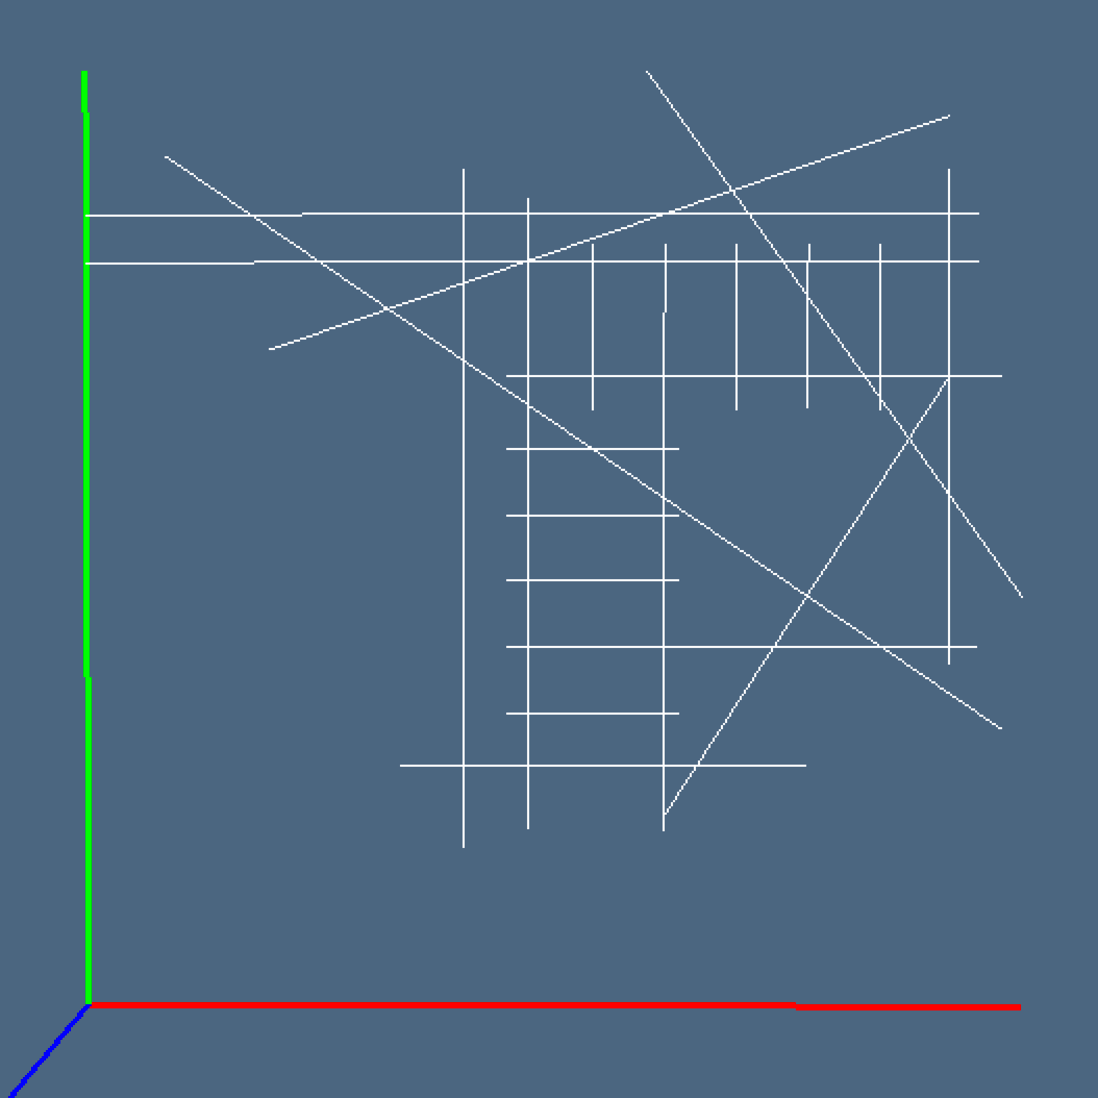
\includegraphics[height=0.2425\linewidth,width=0.2425\linewidth]{images/svg1} 
   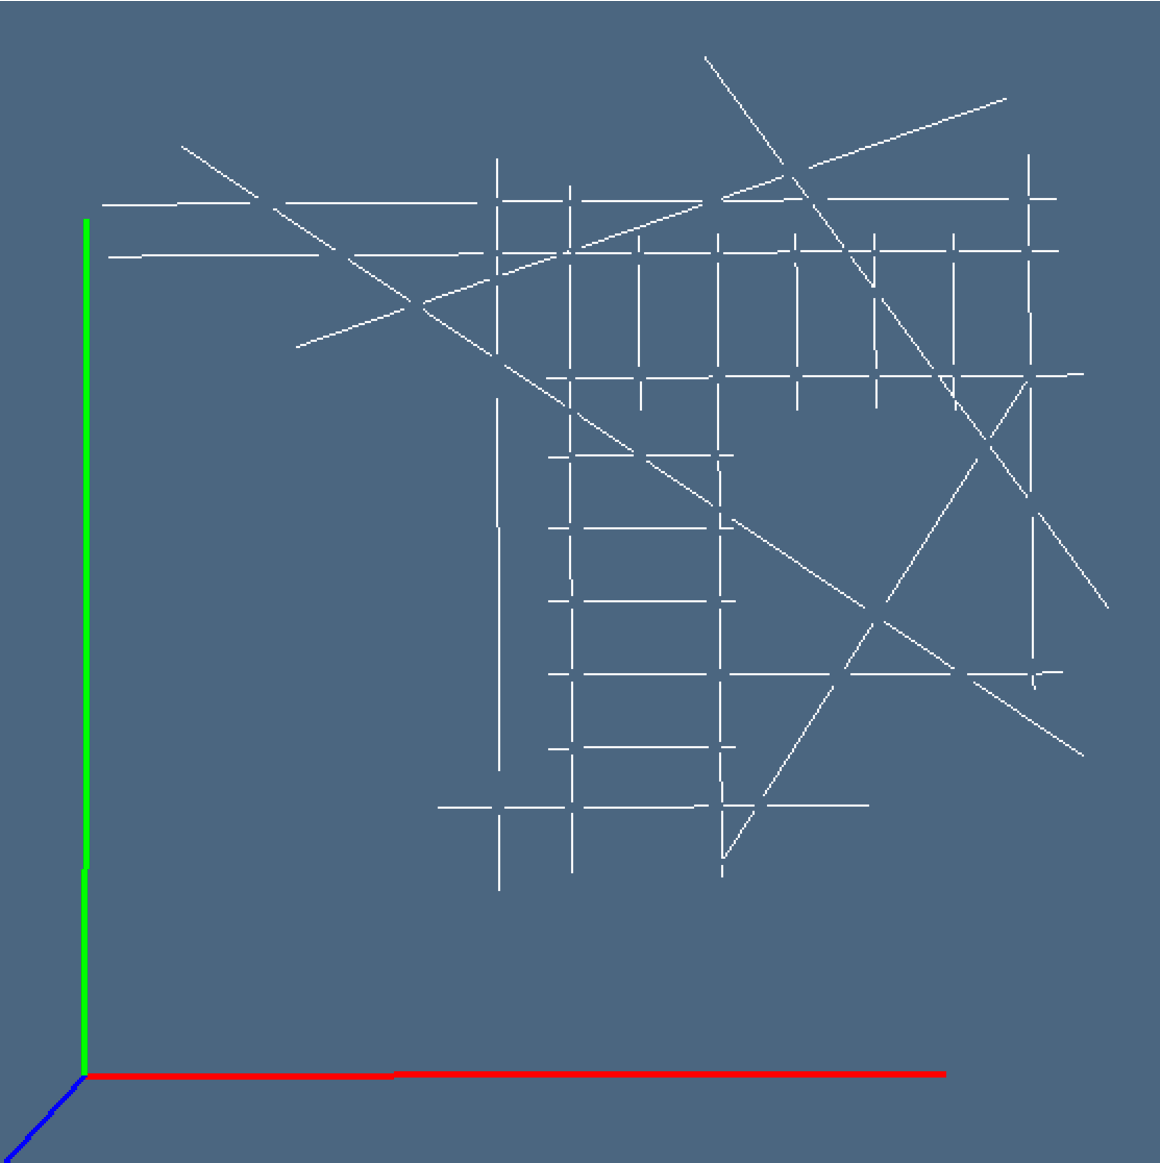
\includegraphics[height=0.2425\linewidth,width=0.2425\linewidth]{images/svg2} 
   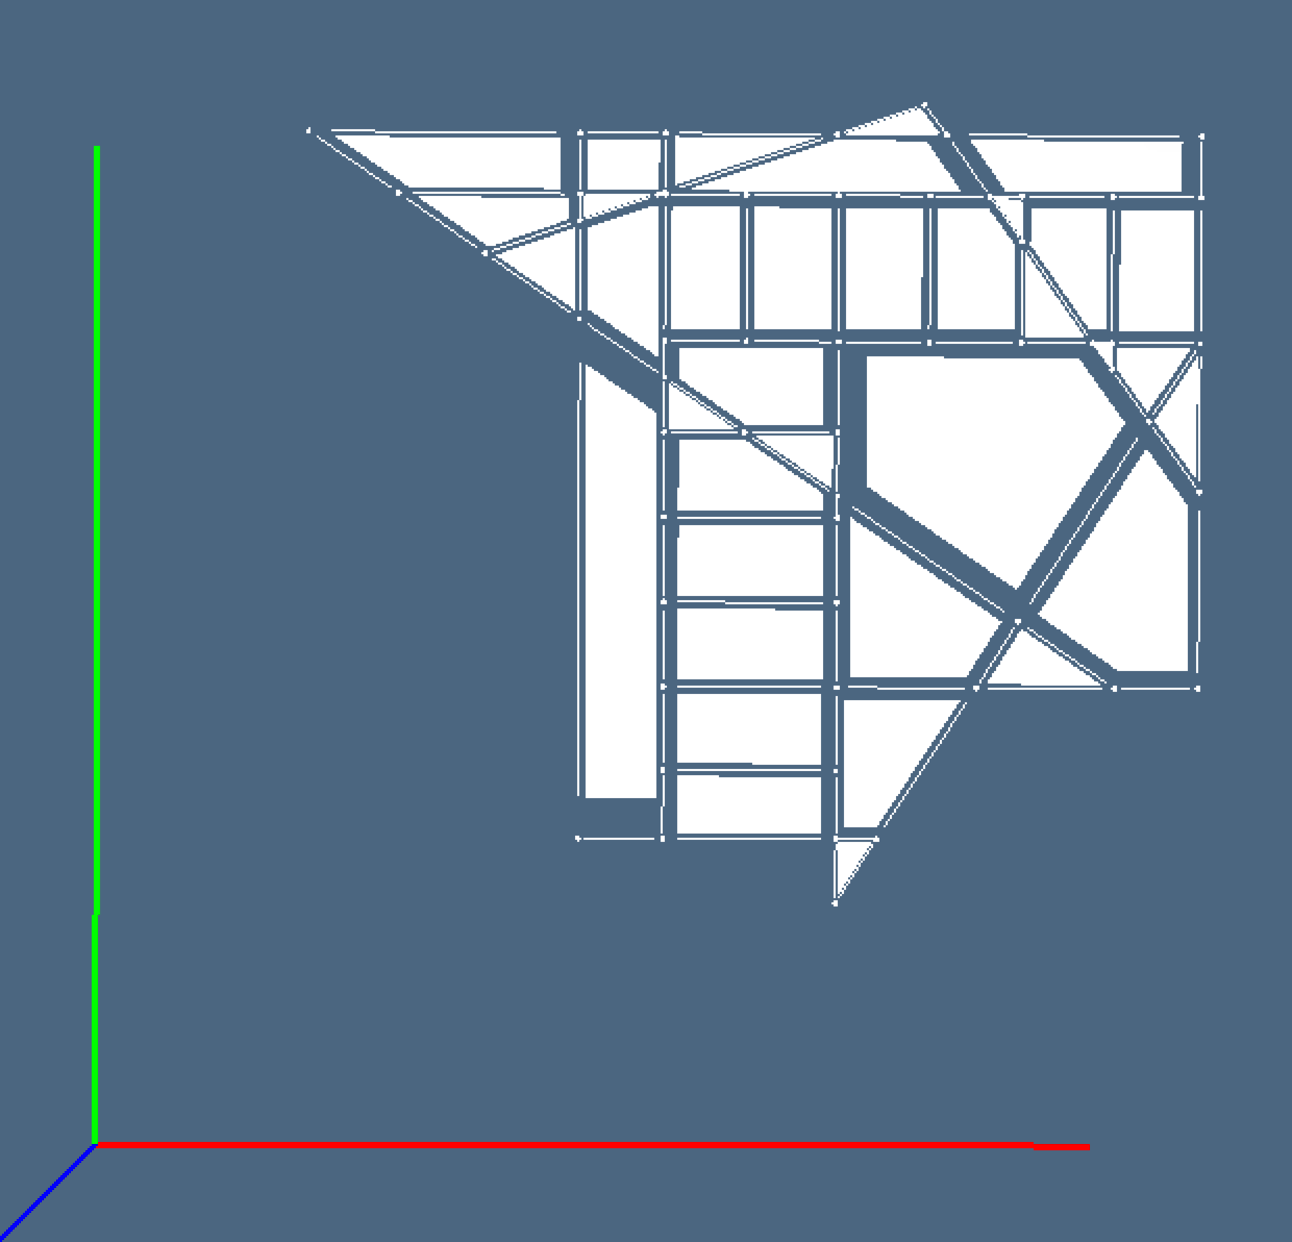
\includegraphics[height=0.2425\linewidth,width=0.2425\linewidth]{images/svg3} 
   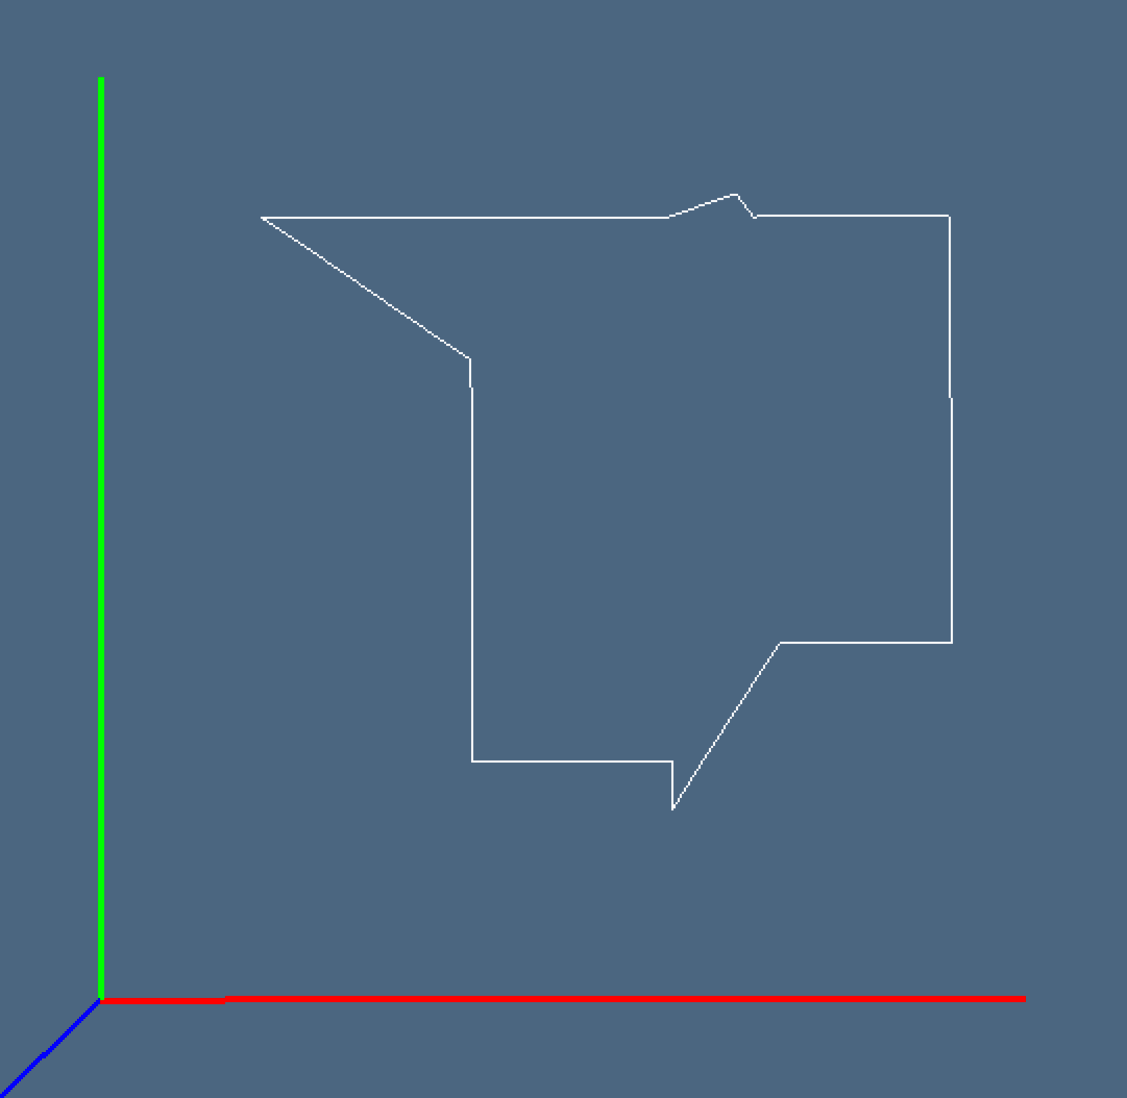
\includegraphics[height=0.2425\linewidth,width=0.2425\linewidth]{images/svg4} 
   \caption{\texttt{LAR} complex generation from \texttt{SVG} file. (a) the input set of lines parsed from an \texttt{SVG} file; (b) the intersection of lines; (c) the extracted \emph{regularized} 2-complex, drawn exploded; (d) the boundary \texttt{LAR}.}
   \label{fig:ortho}
\end{figure}


%-------------------------------------------------------------------------------
@O test/py/inters/test11.py
@{""" Fast Polygon Triangulation based on Seidel's Algorithm """
# data generated by test10.py on file polygon.svg
from larlib import *

V,FV,EV = ([[0.222, 0.889],
  [0.722, 1.0],
  [0.519, 0.763],
  [1.0, 0.659],
  [0.859, 0.233],
  [0.382, 0.119],
  [0.519, 0.348],
  [0.296, 0.53],
  [0.0, 0.059]],
 [[0, 1, 2, 3, 4, 5, 6, 7, 8]],
 [[2, 3], [6, 7], [0, 8], [3, 4], [1, 2], [7, 8], [4, 5], [5, 6], [0, 1]])
 
VV = AA(LIST)(range(len(V)))
submodel = STRUCT(MKPOLS((V,EV)))
VIEW(larModelNumbering(1,1,1)(V,[VV,EV],submodel,0.5))

 
xord = TRANS(sorted(zip(V,range(len(V)))))[1]
trapezoids = zip(xord[:-1],xord[1:])
vert2forw_trap = dict()
vert2back_trap = dict()

for k,(a,b) in enumerate(trapezoids[1:-1]):
    print k,(a,b)
    vert2back_trap[a]=k
    vert2forw_trap[a]=k+1
    vert2back_trap[b]=k+1
    vert2forw_trap[b]=k+2
vert2forw_trap[trapezoids[0][0]] = 0
vert2back_trap[trapezoids[-1][1]] = len(trapezoids)-1
@}
%-------------------------------------------------------------------------------


%-------------------------------------------------------------------------------
@O test/py/inters/test12.py
@{""" Biconnected components from orthogonal LAR model """
from larlib import *

V = [[0.395, 0.296], [0.593, 0.0], [0.79, 0.773], [0.671, 0.889], [0.79, 0.0], [0.593, 0.296], [0.593, 0.593], [0.395, 0.593], [0.0, 0.889], [0.0, 0.0]]
FV = [[0, 5, 4, 1], [1, 9, 0], [8, 7, 0, 9], [7, 8, 3, 2, 4, 5, 6]]
EV = [[0, 1], [8, 9], [6, 7], [4, 5], [1, 4], [3, 8], [5, 6], [2, 3], [1, 9], [0, 9], [0, 5], [0, 7], [7, 8], [2, 4]]
polylines = [[V[v] for v in face+[face[0]]] for face in FV]
VIEW(EXPLODE(1.1,1.1,1)(MKPOLS((V,EV)) + AA(MK)(V) + AA(FAN)(polylines) ))

VV = AA(LIST)(range(len(V)))
submodel = STRUCT(MKPOLS((V,EV)))
VIEW(larModelNumbering(1,1,1)(V,[VV,EV,FV],submodel,.6))

VIEW(EXPLODE(1.1,1.1,1)(AA(POLYLINE)(polylines)))
@}
%-------------------------------------------------------------------------------

\appendix
%===============================================================================
\section{Code utilities}
%===============================================================================

\paragraph{Coding utilities}

Some utility fuctions used by the module are collected in this appendix. Their macro names can be seen in the below script.

%-------------------------------------------------------------------------------
@D Coding utilities
@{""" Coding utilities """
@< Generation of all binary subsets of lenght n @>
@< Generation of a random point @>
@< Generation of a random line segment @>
@< Transformation of a 2D box into a closed polyline @>
@< Computation of the 1D centroid of a list of 2D boxes @>
@< Pyplasm XOR of FAN of ordered points @>
@}
%-------------------------------------------------------------------------------

\paragraph{Generation of all binary subsets of lenght n}

%-------------------------------------------------------------------------------
@D Generation of all binary subsets of lenght n
@{""" Generation of all binary subsets of lenght n """
def allBinarySubsetsOfLenght(n):
	out = [list(('{0:0'+str(n)+'b}').format(k)) for k in range(1,2**n)]
	return AA(AA(int))(out)
@}
%-------------------------------------------------------------------------------

\subparagraph{Example}
\begin{verbatim}
In [9]: allBinarySubsetsOfLenght(3)
Out[9]: [[0,0,1],[0,1,0],[0,1,1],[1,0,0],[1,0,1],[1,1,0],[1,1,1]]
\end{verbatim}


\paragraph{Generation of random lines}
The function \texttt{randomLines} returns the array \texttt{randomLineArray} with a given number of lines generated within the unit 2D interval. The \texttt{scaling} parameter is used to scale every such line, generated by two randow points, that could be possibly located to far from each other, even at the distance of the diagonal of the unit square.

The arrays \texttt{xs} and \texttt{ys}, that contain the $x$ and $y$ coordinates of line points, are used to compute the minimal translation \texttt{v} needed to transport the entire set of data within the positive quadrant of the 2D plane. 

%-------------------------------------------------------------------------------
@D Generation of random lines
@{""" Generation of random lines """
def randomLines(numberOfLines=200,scaling=0.3):
    randomLineArray = [redge(scaling) for k in range(numberOfLines)]
    [xs,ys] = TRANS(CAT(randomLineArray))[:2]
    xmin, ymin = min(xs), min(ys)
    v = array([-xmin,-ymin])
    randomLineArray = [[list(v1[:2]+v), list(v2[:2]+v)] for v1,v2 in randomLineArray]
    return randomLineArray
@}
%-------------------------------------------------------------------------------


\paragraph{Generation of a random point}
A single random point, codified in floating point format, and with a fixed (quite small) number of digits, is returned by the \texttt{rpoint2d()} function, with no input parameters.
%-------------------------------------------------------------------------------
@D Generation of a random point
@{""" Generation of a random point """
def rpoint2d():
    return eval( vcode([ random.random(), random.random() ]) )
@}
%-------------------------------------------------------------------------------
    
\paragraph{Generation of a random line segment}
A single random segment, scaled about its centroid by the \texttt{scaling} parameter, is returned by the \texttt{redge()} function, as a tuple ot two random points in the unit square.
%-------------------------------------------------------------------------------
@D Generation of a random line segment
@{""" Generation of a random line segment """
def redge(scaling):
    v1,v2 = array(rpoint2d()), array(rpoint2d())
    c = (v1+v2)/2
    pos = rpoint2d()
    v1 = (v1-c)*scaling + pos
    v2 = (v2-c)*scaling + pos
    return tuple(eval(vcode(v1))), tuple(eval(vcode(v2)))
@}
%-------------------------------------------------------------------------------
    
\paragraph{Transformation of a 2D box into a closed polyline}
The transformation of a 2D box into a closed rectangular polyline, given as an ordered sequwncw of 2D points, is produced by the function \texttt{box2rect}
%-------------------------------------------------------------------------------
@D Transformation of a 2D box into a closed polyline
@{""" Transformation of a 2D box into a closed polyline """    
def box2rect(box):
    x1,y1,x2,y2 = box
    verts = [[x1,y1],[x2,y1],[x2,y2],[x1,y2],[x1,y1]]
    return verts
@}
%-------------------------------------------------------------------------------
    
\paragraph{Computation of the 1D centroid of a list of 2D boxes}
The 1D \texttt{centroid} of a list of 2D boxes is computed by the function given below.
The direction of computation (either $x$ or $y$) is chosen depending on the value of the \texttt{xy} parameter. 
%-------------------------------------------------------------------------------
@D Computation of the 1D centroid of a list of 2D boxes
@{""" Computation of the 1D centroid of a list of 2D boxes """    
def centroid(boxes,coord):
    delta,n = 0,len(boxes)
    ncoords = len(boxes[0])/2
    a = coord%ncoords
    b = a+ncoords
    for box in boxes:
        delta += (box[a] + box[b])/2
    return delta/n

@}
%-------------------------------------------------------------------------------


\paragraph{Pyplasm XOR of FAN of ordered points}

%-------------------------------------------------------------------------------
@D Pyplasm XOR of FAN of ordered points
@{""" XOR of FAN of ordered points """ 
def FAN(points): 
    pairs = zip(points[1:-2],points[2:-1])
    triangles = [MKPOL([[points[0],p1,p2],[[1,2,3]],None]) for p1,p2 in pairs]
    return XOR(triangles)
 
if __name__=="__main__":
    pol = [[0.476,0.332],[0.461,0.359],[0.491,0.375],[0.512,0.375],[0.514,0.375],
    [0.527,0.375],[0.543,0.34],[0.551,0.321],[0.605,0.314],[0.602,0.307],[0.589,
    0.279],[0.565,0.244],[0.559,0.235],[0.553,0.227],[0.527,0.239],[0.476,0.332]]

    VIEW(EXPLODE(1.2,1.2,1)(FAN(pol)))
@}
%-------------------------------------------------------------------------------


\bibliographystyle{amsalpha}
\bibliography{inters}

\end{document}
